% XeLatex编辑
\documentclass[10pt, a4paper]{article}

\usepackage{ucas_matrix}

\begin{document}

\ucascover

% --- 目录 ---
% 会自动生成带“目录”标题的目录页
\tableofcontents
\newpage

% --- 正文开始 ---

\section{矩阵与线性方程组}

\subsection{线性方程组}

\subsubsection{高斯消元法和矩阵}

\subsubsection{高斯-约当消元法}

\subsubsection{MAKING GAUSSIAN ELIMINATION WORK}
\subsection{一般线性系统与阶梯形式}

\subsubsection{高斯消去法的改进与行阶梯型(Row Echelon Form)}

\subsubsection{行简化阶梯形矩阵(REDUCED ROW ECHELONFORM)}
\subsection*{2.3 线性方程组的一致性(Consistency Of Linear Systems)}

如果一个包含 \(n\) 个未知数的 \(m\) 个线性方程组至少有一个解,则称其为相容方程组。如果没有解,则该方程组
被称为不相容方程组。本节旨在确定给定方程组相容的条件。

对于仅包含两个或三个未知数的方程组,
说明其相容性条件很容易。两个未知数的线性方程表示二维空间中的一条直线,
而三个未知数的线性方程表示三维空间中的平面。因此,
一个包含 \(m\) 个两个未知数的线性方程组相容当且仅当这 \(m\) 个方程定义的 \(m\) 条直线至少有一个公共交点。
同样,一个包含 \(m\) 个三个未知数的方程组相容当且仅当
相关的 \(m\) 个平面至少有一个公共交点。
然而,当 \(m\) 较大时,这些几何条件可能不易直观验证,而当 \(n\) > 3 时,相交线或平面的推广则无法用肉眼直观地看到。

我们不依赖几何来建立一致性,而是使用高斯消元法。如果将相关的增广矩阵 \([A|b]\) 通过行运算简化为行阶梯矩阵 \([E|c]\),则一致性(或不一致性)变得显而易见。
假设在将 \([A|b]\) 简化为 \([E|c]\) 的过程中,出现这样一种情况:一行中唯一的非零项出现在右侧,如下所示:

\[
\mathrm{Row}\_i \rightarrow 
\left(\begin{array}{cccccc|c}
* & * & * & * & * & * & * \\ 
0 & 0 & 0 & * & * & * & * \\ 
0 & 0 & 0 & 0 & 0 & 0 & \alpha \\
\bullet & \bullet & \bullet & \bullet & \bullet & \bullet & \bullet \\
\bullet & \bullet & \bullet & \bullet & \bullet & \bullet & \bullet \\
\end{array}\right)
\leftarrow \alpha \neq 0.
\]

如果这发生在第 i 行,则相关系统的第 i 个方程为

\[
0x_1 + 0x_2 + ... + 0x_n = \alpha.
\]

当 \(\alpha \neq 0\) 时,该方程无解,因此原系统也必然不一致(因为行运算不会改变解集)。
反之亦然。也就是说,如果一个系统不一致,那么在消元过程中,会出现如下形式的行

\[
\left(\begin{array}{cccccc|c}
0 & 0 & ... & 0 & \alpha
\end{array}\right), \alpha \neq 0.
\]

否则,回代过程可以完成,并产生一个解。当遇到形式为
(0 0 ... 0 \(\mid\) 0) 的行时,不会指示不一致性。这只是表示 0 = 0,
尽管这对于确定任何未知数的值没有任何帮助,但它仍然是一个真实的陈述,
因此它并不表示系统存在不一致。

还有一些其他方法可以表征系统的一致性(或不一致性)。其中一种方法是:如果增广矩阵 \([A|b]\) 的最后一列 \(b\) 是非基列,则最后一列不可能存在主元,因此系统是一致的,因为 (2.3.1) 的情况不会发生。
反之,如果系统是一致的,那么 (2.3.1) 的情况在高斯消元法中永远不会发生,因此最后一列不可能是基列。换句话说,\([A|b]\) 是一致的当且仅当 \(b\) 是非基列。

说 b 是 \([A|b]\) 中的非基列,等同于说\([A|b]\) 中的所有基列都位于系数矩阵 A 中。由于矩阵中基列的数量就是秩,因此一致性也可以这样来描述:
当且仅当 rank\([A|b]\) = rank\((A)\) 时,系统才是一致的。



\begin{bluebox}{线性方程组的一致性}
满足以下任意一个条件都可以说 \([A|b]\) 是一致的:
\begin{itemize}
    \item 行简化阶梯形矩阵 \([A|b]\) 中不存在形如下列的行:
    \[
    \left(\begin{array}{cccc|c}
        0 & 0 & ... & 0 & \alpha
    \end{array}\right), \alpha \neq 0
    \]
    \item \(b\) 是 \([A|b]\) 中的非基列。
    \item rank\([A|b]\) = rank\((A)\)
    \item \(b\) 是 \(A\) 的基列的一个组合。
\end{itemize}
\end{bluebox}

% 红色文字
\textcolor{red}{例子2.3.1}
% 红色水平线(宽度为文本宽度,厚度0.4pt)
\color{red}\rule{\textwidth}{0.4pt}\color{black}

\textbf{问题}: 确定以下系统是否一致: 
\[
\begin{align} 
    x_1 + x_2 + 2x_3 + 2x_4 + x_5 = 1, \\
    2x_1 + 2x_2 + 4x_3 + 4x_4 + 3x_5 = 1, \\
    2x_1 + 2x_2 + 4x_3 + 4x_4 + 2x_5 = 2, \\
    3x_1 + 5x_2 + 8x_3 + 6x_4 + 5x_5 = 3.
\end{align}
\]
\textbf{解答}: 对增广矩阵 \([A|b]\) 应用高斯消元法,如下所示
\[
\left(\begin{array}{ccccc|c} 
\circlednum{1} & 1 & 2 & 2 & 1 & 1 \\ 
2 & 2 & 4 & 4 & 3 & 1 \\ 
2 & 2 & 4 & 4 & 2 & 2 \\ 
3 & 5 & 8 & 6 & 5 & 3 
\end{array}\right)
\to
\left(\begin{array} {ccccc|c} 
\circlednum{1} & 1 & 2 & 2 & 1 & 1 \\ 
0 & \circlednum{0} & 0 & 0 & 1 & -1 \\ 
0 & 0 & 0 & 0 & 0 & 0 \\ 
0 & 2 & 2 & 0 & 2 & 0 
\end{array}\right)
\to
\left(\begin{array}{ccccc|c} 
\circlednum{1} & 1 & 2 & 2 & 1 & 1 \\ 
0 & \circlednum{2} & 2 & 0 & 2 & 0 \\ 
0 & 0 & 0 & 0 & \circlednum{1} & -1 \\ 
0 & 0 & 0 & 0 & 0 & 0 
\end{array}\right)
\]

由于形式为 \left(\begin{array}{cccc|c} 0 & 0 & ... & 0 & \alpha \end{array}\right), 
\(\alpha \neq 0\) 的行从未出现,
因此系统是一致的。我们还可以观察到,\(b\) 是 \([A|b]\) 中的非基本列,
因此 rank\([A|b]\) = rank \((A)\)。最后,通过将 \(A\) 完全约化为
\(E_A\),可以验证 \(b\) 确实是基本列的组合,\{\(A_{*1}, A_{*2}, A_{*5}\)\}。

% 红色文字
\textcolor{red}{练习 2.3}
% 红色水平线(宽度为文本宽度,厚度0.4pt)
\color{red}\rule{\textwidth}{0.4pt}\color{black}

\begin{enumerate}[leftmargin=*, label=\bfseries 2.3.\arabic*]

\item Determine which of the following systems are consistent.

\begin{enumerate}[label=(\alph*)]
    \item \(\begin{array}{l}
    x + 2y + z = 2, \\
    2x + 4y = 4, \\
    3x + 6y + z = 4.
    \end{array}\)
    
    \item \(\begin{array}{l}
    2x + 2y + 4z = 0, \\
    3x + 2y + 5z = 0, \\
    4x + 2y + 6z = 0.
    \end{array}\)
    
    \item \(\begin{array}{l}
    x - y + z = 1, \\
    x - y - z = 2, \\
    x + y - z = 3, \\
    x + y + z = 4.
    \end{array}\)

    \item \(\begin{array}{l}
    x - y + z = 1, \\
    x - y - z = 2, \\
    x + y - z = 3, \\
    x + y + z = 2.
    \end{array}\)

    \item \(\begin{array}{l}
    2w + x + 3y + 5z = 1, \\
    4w + 4y + 8z = 0, \\
    w + x + 2y + 3z = 0, \\
    x + y + z = 0.
    \end{array}\)

    \item \(\begin{array}{l}
    2w + x + 3y + 5z = 7, \\
    4w + 4y + 8z = 8, \\
    w + x + 2y + 3z = 5, \\
    x + y + z = 3.
    \end{array}\)
\end{enumerate}

\item Construct a \(3 \times 4\) matrix \(A\) and \(3 \times 1\) columns \(b\) and \(c\) such that \([A|b]\) is the augmented matrix for an inconsistent system, but \([A|c]\) is the augmented matrix for a consistent system.

\item If \(A\) is an \(m \times n\) matrix with rank\((A) = m\), explain why the system \([A|b]\) must be consistent for every right-hand side \(b\).

\item Is it possible for a parabola whose equation has the form \(y = \alpha+\beta x+\gamma x^2\) to pass through the four points (0, 1), (1, 3), (2, 15), and (3, 37)? Why?

\item Consider using floating-point arithmetic (without scaling) to solve the following system:
\[
\begin{array}{l}
.835x + .667y = .168, \\
.333x + .266y = .067.
\end{array}
\]
\begin{enumerate}[label=(\alph*)]
    \item Is the system consistent when 5-digit arithmetic is used?
    
    \item What happens when 6-digit arithmetic is used?
\end{enumerate}

\item In order to grow a certain crop, it is recommended that each square foot of ground be treated with 10 units of phosphorous, 9 units of potassium, and 19 units of nitrogen. 
Suppose that there are three brands of fertilizer on the market— say brand \(\mathcal{X}\) , brand \(\mathcal{Y}\) , and brand \(\mathcal{Z}\).
One pound of brand \(\mathcal{X}\) contains 2 units of phosphorous, 3 units of potassium, and 5 units of nitrogen. One pound of brand \(\mathcal{Y}\) contains 1 unit of phosphorous,
3 units of potassium, and 4 units of nitrogen. One pound of brand \(\mathcal{Z}\) contains only 1 unit of phosphorous and 1 unit of nitrogen.
Determine whether or not it is possible to meet exactly the recommendation by applying some combination of the three brands of fertilizer.

\item Suppose that an augmented matrix \([A|b]\) is reduced by means of Gaussian elimination to a row echelon form \([E|c]\). If a row of the form 
\[
\left(\begin{array}{cccc|c}
    0 & 0 & ... & 0 & \alpha
\end{array}\right), \alpha \neq 0
\]
does not appear in \([E|c]\), is it possible that rows of this form could have appeared at earlier stages in the reduction process? Why?

\end{enumerate}

\subsection*{2.4 齐次系统(Homogeneous Systems)}

\(n\) 个未知数的 \(m\) 个线性方程组
\[
\begin{array}{cols}
    a_{11}x_1 + a_{12}x_2 + ... + a_{1n}x_n = 0, \\
    a_{21}x_1 + a_{22}x_2 + ... + a_{2n}x_n = 0, \\
    \vdots \\
    a_{m1}x_1 + a_{m2}x_2 + ... + a_{mn}x_n = 0.
\end{array}
\]

如果方程式的右侧完全由0组成,则称其为\textbf{齐次系统}。如果方程式的右侧至少有一个非零数,则该系统称为\textbf{非齐次系统}。本节旨在探讨齐次系统的一些基本概念。

在处理齐次方程组时,一致性从来都不是问题,因为无论系数值如何,
零解 \(x_1 = x_2 = ... = x_n = 0\) 始终是唯一解。下文中,
将全零组成的解称为\textbf{平凡解}。唯一的问题是:“除了平凡解之外,还有其他解吗?
如果有,我们如何才能最好地描述它们?” 和之前一样,高斯消元法可以给出答案。

使用高斯消元法将齐次系统的增广矩阵 \([A|0]\) 化简为行阶梯形时,右侧的零列不会被任何三种基本行运算改变。
也就是说,任何通过行运算从 \([A|0]\) 导出的行阶梯形,也必然具有 \([E|0]\) 的形式。这意味着最后一列的零只是
多余的负担,没有必要在每一步都带上去。只需将系数矩阵 \(A\) 化简为行阶梯形 \(E\),并记住在执行回代时,右侧
完全为零。通过一个典型的例子,可以更好地理解这个过程。

为了求解齐次系统的解
\[
\begin{array}{cols}
    x_1 + 2x_2 + 2x_3 + 3x_4 = 0, \\
    2x_1 + 4x_2 + x_3 + 3x_4 = 0, \\
    3x_1 + 6x_2 + x_3 + 4x_4 = 0,
\end{array}
\]
将系数矩阵简化为行阶梯形式。
\[
A = 
\left(\begin{array}{cccc}
1 & 2 & 2 & 3 \\
2 & 4 & 1 & 3 \\
3 & 6 & 1 & 4
\end{array}\right)\to
\left(\begin{array}{cccc}
1 & 2 & 2 & 3 \\
0 & 0 & -3 & -3 \\
0 & 0 & -5 & -5
\end{array}\right)\to
\left(\begin{array}{cccc}
1 & 2 & 2 & 3 \\
0 & 0 & -3 & -3 \\
0 & 0 & 0 & 0
\end{array}\right)
= E
\]
因此,原始齐次系统等价于以下简化齐次系统:
\[
\begin{array}{cols}
    x_1 + 2x_2 + 2x_3 + 3x_4 = 0, \\
    -3x_3 - 3x_4 = 0.
\end{array}
\]
由于这个简化系统中有四个未知数,但只有两个方程,因此不可能为每个未知数求出唯一的解。我们能做的最好的事情是,
选择两个“基本”未知数——我们称之为\textbf{基本变量},并用另外两个未知数来求解它们——这两个未知数的值必须
保持任意或“自由”,因此它们被称为\textbf{自由变量}。虽然选择一组基本变量有多种可能性,但惯例是始终求解与枢轴位置对应的未知数,
或者,等价地,与基本列对应的未知数。在这个例子中,枢轴(以及基本列)位于第一和第三位置,
因此策略是应用回代法,用自由变量 \(x_2\) 和 \(x_4\) 来求解简化系统中的基本变量 \(x_1\) 和 \(x_3\)。由第二个方程得出
\[
x_3 = -x_4.
\]
代入第一个方程可得
\[
\begin{align}
x_1 &= -2x_2 -2x_3 - 3x_4, \\
&= -2x_2 - 2(-x_4) - 3x_4, \\
&= -2x_2 - x_4.
\end{align}
\]
因此,原齐次系统的所有解都可以描述为
\[
\begin{align}
    &x_1 = -2x_2 - x_4 \\
    &x_2 \text{ "free"}, \\
    &x_3 = -x_4, \\
    &x_4 \text{ "free"}.
\end{align}
\]
由于自由变量 \(x_2\) 和 \(x_4\) 取值范围涵盖所有可能值,上述表达式描述了所有可能的解。例如,当 \(x_2\) 和 \(x_4\) 取值
\(x_2\) = 1 且 \(x_4\) = -2 时,则有特定解
\[
x_1 = 0, x_2 = 1, x_3 = 2, x_4 = -2
\]
将来不再像上述那样描述解集,而是更方便地通过以下方式表达解集: 
\[
\left(\begin{array}{cols}
x_1\\
x_2\\
x_3\\
x_4
\end{array}\right)=
\left(\begin{array}{cols}
-2x_2 - x_4\\
x_2\\
-x_4\\
x_4
\end{array}\right)=
x_2\left(\begin{array}{cols}
-2\\
1\\
0\\
0
\end{array}\right)+
x_4\left(\begin{array}{cols}
-1\\
0\\
-1\\
1
\end{array}\right)
\]
假设 \(x_2\) 和 \(x_4\) 是自由变量,其取值范围为所有可能的数字。这种表示被称为齐次系统的\textbf{通解}。
通解的表达式强调,每个解都是两个特解的某种组合
\[
h_1 = 
\left(\begin{array}{cols}
-2\\
1\\
0\\
0
\end{array}\right),  
h_2 =
\left(\begin{array}{cols}
-1\\
0\\
-1\\
1
\end{array}\right).
\]
\(h_1\) 和 \(h_2\) 显然都是解,因为 \(h_1\) 是在自由变量取值 \(x_2\) = 1 和 \(x_4\) = 0 时生成的,而
解 \(h_2\) 是在 \(x_2\) = 0 和 \(x_4\) = 1 时生成的。

现在考虑一个由 \(m\) 个线性方程组 \([A|0]\) 组成的广义齐次方程组,
其中有 \(n\) 个未知数。如果系数矩阵的 rank(\(A\)) = \(r\),那么
从前面的讨论中应该可以明显看出,恰好有 \(r\) 个
基本变量(对应于 \(A\) 中基本列的位置),以及
恰好有 \(n - r\) 个自由变量(对应于 \(A\) 中非基本列的位置)。
使用高斯消元法将 \(A\) 化为行阶梯形,
然后使用回代法根据自由变量求解基本变量,
即可得到\textbf{通解},其形式为
\[
\mathrm{x} = x_{f_1}\mathrm{h}_1 + x_{f_2}\mathrm{h}_2 + ... + x_{f_{n-r}}\mathrm{h}_{n-r},
\]
其中 \(x_{f_1}, x_{f_2}, ..., x_{f_{n-r}}\) 为自由变量,\(h_1, h_2, ..., h_{n-r}\) 为
\(n \times 1\) 列,表示系统的特定解。由于自由变量 \(x_{f_i}\) 涵盖所有可能值,因此通解会生成所有可能的解。

通解并不依赖于所用的行阶梯形式,因为无论使用哪种行阶梯形式,使用回代法求解基本变量,都会生成一组唯一的特解,
{\(h_1, h_2, ..., h_{n-r}\)}。无需赘述,我们可以认为这是正确的,因为使用任何行阶梯形式求解基本变量,
其结果必然与将 \(A\) 完全简化为 \(E_A\),然后求解简化齐次系统的基本变量,所得结果完全相同。\(E_A\) 的唯一性,保证了 \(h_i\) 的唯一性。

例如,如果与第一个系统相关的系数矩阵 \(A\) 通过高斯-乔丹方法完全简化为 \(E_A\)
\[
A = 
\left(\begin{array}{cccc}
    1 & 2 & 2 & 3 \\
    2 & 4 & 1 & 3 \\
    3 & 6 & 1 & 4 \\
\end{array}\right)\to
\left(\begin{array}{cccc}
    1 & 2 & 0 & 1 \\
    0 & 0 & 1 & 1 \\
    0 & 0 & 0 & 0 \\
\end{array}\right)= E_A
\]
然后我们得到以下简化系统:
\[
\begin{align}
    x_1 + 2x_2 + x_4 &= 0, \\
    x_3 + x_4 &= 0.
\end{align}
\]
用 \(x_2\) 和 \(x_4\) 来求解基本变量 \(x_1\) 和 \(x_3\),得到的结果与当时的推导给出的结果完全相同,因此也得到了与后续的通解完全相同的结果。

由于避免了回代过程,你可能会发现使用高斯-约当法将 \(A\) 完全简化为 \(E_A\) 更为方便,
然后直接从 \(E_A\) 中的元素构建通解。这种方法通常会在示例和练习中采用。

如前所述,所有齐次系统都是一致的,因为由全零组成的平凡解始终是唯一解。一个自然而然的问题是:“平凡解何时是唯一解?”
换句话说,我们想知道齐次系统何时具有唯一解。上述的形式使答案显而易见。只要至少有一个自由变量,那么从上述可以清楚地看出,
将存在无数个解。因此,当且仅当没有自由变量时,平凡解才是唯一解。
由于自由变量的数量为 \(n - r\),其中 \(r\) = rank(\(A\)),因此前面的陈述可以重新表述为:当且仅当 rank(\(A\)) = \(n\),齐次系统才具有唯一解——平凡解。

% 红色文字
\textcolor{red}{例子2.4.1}
% 红色水平线(宽度为文本宽度,厚度0.4pt)
\color{red}\rule{\textwidth}{0.4pt}\color{black}

齐次系统
\[
\begin{align} 
    x_1 + 2x_2 + 2x_3 = 0, \\
    2x_1 + 5x_2 + 7x_3 = 0, \\
    3x_1 + 6x_2 + 8x_3 = 0.
\end{align}
\]
只有平凡解因为
\[
A = 
\left(\begin{array}{ccc}
    1 & 2 & 2 \\
    2 & 5 & 7 \\
    3 & 6 & 8 \\
\end{array}\right)\to
\left(\begin{array}{cccc}
    1 & 2 & 2 \\
    0 & 1 & 3 \\
    0 & 0 & 2 \\
\end{array}\right) = E
\]
表明 rank(\(A\)) = \(n\) = 3。事实上,从 \(E\) 中也可以看出,在系统 \([E|0]\) 中应用反向替换只会产生平凡解。

% 红色文字
\textcolor{red}{例子2.4.2}
% 红色水平线(宽度为文本宽度,厚度0.4pt)
\color{red}\rule{\textwidth}{0.4pt}\color{black}

\textbf{问题}: 解释为什么下列齐次系统有无穷多个解,并给出通解:
\[
\begin{align} 
    x_1 + 2x_2 + 2x_3 = 0, \\
    2x_1 + 5x_2 + 7x_3 = 0, \\
    3x_1 + 6x_2 + 6x_3 = 0.
\end{align}
\]
\textbf{解答}: 
\[
A = 
\left(\begin{array}{ccc}
    1 & 2 & 2 \\
    2 & 5 & 7 \\
    3 & 6 & 6 \\
\end{array}\right)\to
\left(\begin{array}{cccc}
    1 & 2 & 2 \\
    0 & 1 & 3 \\
    0 & 0 & 0 \\
\end{array}\right) = E
\]
表明 rank(\(A\)) = 2 < \(n\) = 3。由于基本列位于位置1 和 2,\(x_1\) 和 \(x_2\) 是基本变量,而 \(x_3\) 是自由变量。使用
\([E|0]\) 的反向代入,用自由变量来求解基本变量,可得 \(x_2 = -3x_3\) 和 \(x_1 = -2x_2 - 2x_3 = 4x_3\),因此通解为
\[
\left(\begin{array}{c}
    x_1 \\
    x_2 \\
    x_3 \\
\end{array}\right) = x_3
\left(\begin{array}{c}
    4 \\
    -3 \\
    1 \\
\end{array}\right), \text{其中} x_3 \text{是自由变量}.
\]
也就是说,每个解都是一个特定解 \(h_1 = \left(\begin{array}{cols} 4 \\-3 \\1\end{array}\right)\) 的倍数

\begin{bluebox}{总结}
设 \(A_{m \times n}\) 为 \(m\) 个齐次线性方程组的系数矩阵,其中 \(n\) 个未知数,并设 rank(\(A\)) = \(r\)。
\begin{itemize}
    \item 与基本列的位置(即枢轴位置)相对应的未知数称为\textbf{基本变量},与非基本列的位置相对应的未知数称为\textbf{自由变量}。
    \item 恰好有 \(r\) 个基本变量和 \(n-r\) 个自由变量。
    \item 为了描述所有解,使用高斯消元法将 \(A\) 化为行阶梯形式,然后使用回代法求解,以自由变量的形式表示基本变量。这样就得到了通解,其形式为
    \[
    \mathrm{x} = x_{f_1}\mathrm{h}_1 + x_{f_2}\mathrm{h}_2 + ... + x_{f_{n-r}}\mathrm{h}_{n-r},
    \]
    其中 \(x_{f_1}, x_{f_2}, ..., x_{f_{n-r}}\) 为自由变量,\(h_1, h_2, ..., h_{n-r}\) 为 \(n \times 1\) 列,表示齐次方程组的特解。\(h_i\) 与回代过程中使用的
    行阶梯形式无关。由于自由变量 \(x_{f_i}\) 涵盖所有可能值,因此通解会生成所有可能的解。
    \item 一个齐次系统拥有唯一解(平凡解),当且仅当 rank(\(A\)) = \(n\) ——即当且仅当不存在自由变量。
\end{itemize}
\end{bluebox}


% 红色文字
\textcolor{red}{练习 2.4}
% 红色水平线(宽度为文本宽度,厚度0.4pt)
\color{red}\rule{\textwidth}{0.4pt}\color{black}

\begin{enumerate}[leftmargin=*, label=\bfseries 2.4.\arabic*]

\item Determine the general solution for each of the following homogeneous systems.

\begin{enumerate}[label=(\alph*)]
    \item \(\begin{array}{l}
    x_1 + 2x_2 + x_3 + 2x_4 = 0, \\
    2x_1 + 4x_2 + x_3 + 3x_4 = 0, \\
    3x_1 + 6x_2 + x_3 + 4x_4 = 0.
    \end{array}\)
    
    \item \(\begin{array}{l}
    2x + y + z = 0, \\
    4x + 2y + z = 0, \\
    6x + 3y + z = 0, \\
    8x + 4y + z = 0.
    \end{array}\)
    
    \item \(\begin{array}{l}
    x_1 + x_2 + 2x_3 = 0, \\
    3x_1 + 3x_3 + 3x_4 = 0, \\
    2x_1 + x_2 + 3x_3 + x_4 = 0. \\
    x_1 + 2x_2 + 3x_3 - x_4 = 0,
    \end{array}\)

    \item \(\begin{array}{l}
    2x + y + z = 0, \\
    4x + 2y + z = 0, \\
    6x + 3y + z = 0, \\
    8x + 5y + z = 0.
    \end{array}\)
\end{enumerate}

\item Among all solutions that satisfy the homogeneous system
\[
\begin{align}
x + 2y + z &= 0, \\
2x + 4y + z &= 0, \\
x + 2y - z &=0.
\end{align}
\]
determine those that also satisfy the nonlinear constraint \(y - xy = 2z\).

\item Consider a homogeneous system whose coefficient matrix is
\[
A = \left(\begin{array}{ccccc}
    1 & 2 & 1 & 3 & 1 \\
    2 & 4 & -1 & 3 & 8 \\
    1 & 2 & 3 & 5 & 7 \\
    2 & 4 & 2 & 6 & 2 \\
    3 & 6 & 1 & 7 & -3
\end{array}\right).
\]
First transform \(A\) to an unreduced row echelon form to determine the
general solution of the associated homogeneous system. Then reduce \(A\)
to \(E_A\), and show that the same general solution is produced.

\item If \(A\) is the coefficient matrix for a homogeneous system consisting of four equations in eight unknowns and if there are five free variables, what is rank(\(A\))?

\item Suppose that \(A\) is the coefficient matrix for a homogeneous system of four equations in six unknowns and suppose that \(A\) has at least one nonzero row.
\begin{enumerate}[label=(\alph*)]
    \item Determine the fewest number of free variables that are possible.
    \item Determine the maximum number of free variables that are possible.
\end{enumerate}

\item Explain why a homogeneous system of \(m\) equations in \(n\) unknowns where \(m < n\) must always possess an infinite number of solutions.

\item Construct a homogeneous system of three equations in four unknowns that has
\[
x_2\left(\begin{array}{cols}
    -2 \\
    1 \\
    0 \\
    0
\end{array}\right)+
x_4\left(\begin{array}{cols}
    -1 \\
    0 \\
    -1 \\
    1
\end{array}\right)
\]
as its general solution.

\item If \(c_1\) and \(c_2\) are columns that represent two particular solutions of the same homogeneous system, explain why the sum \(c_1 + c_2\) must also represent a solution of this system.

\end{enumerate}

% 定义画圈命令,用于标记主元
\newcommand{\circlednum}[1]{%
    \tikz[baseline=(char.base)]{%
        \node[draw, circle, inner sep=1pt] (char) {#1};%
    }%
}

\section*{2.5 非齐次系统}
回忆一下,一个包含 \(m\) 个线性方程和 \(n\) 个未知数的系统
\[
a_{11}x_{1} + a_{12}x_{2} + \cdots + a_{1n}x_{n} = b_{1}, \quad
a_{21}x_{1} + a_{22}x_{2} + \cdots + a_{2n}x_{n} = b_{2}, \quad \ldots, \quad
a_{m1}x_{1} + a_{m2}x_{2} + \cdots + a_{mn}x_{n} = b_{m}
\]
当至少有一个 \(b_{i} \neq 0\) 时,被称为非齐次系统。与齐次系统不同,非齐次系统可能是不一致的,因此必须应用 §2.3 的技术来判断解是否存在。除非特别说明,本节假设所有系统都是一致的。

为了描述一致非齐次系统的所有可能解,采用与齐次系统相同的方法构造通解:
- 使用高斯消元法将增广矩阵 \([A \mid b]\) 化简为行阶梯形式 \([E \mid c]\)。
- 识别基本变量和自由变量,方法如 §2.4 所述。
- 对 \([E \mid c]\) 应用回代法,将基本变量用自由变量表示。
- 将结果写成形式
  \[
  x = p + x_{f_{1}} h_{1} + x_{f_{2}} h_{2} + \cdots + x_{f_{n-r}} h_{n-r},
  \]
  其中 \(x_{f_{1}}, x_{f_{2}}, \ldots, x_{f_{n-r}}\) 是自由变量,而 \(p, h_{1}, h_{2}, \ldots, h_{n-r}\) 是 \(n \times 1\) 列向量。这就是非齐次系统的通解。

当自由变量 \(x_{f_{i}}\) 取所有可能值时,通解 (2.5.1) 生成系统 \([A \mid b]\) 的所有可能解。与齐次情况类似,列 \(h_{i}\) 和 \(p\) 不依赖于所使用的行阶梯形式 \([E \mid c]\)。因此,可以通过高斯-约当法将 \([A \mid b]\) 完全化简为 \(E_{[A \mid b]}\),从而避免回代过程。在方便时,我们将采用这种方法。

非齐次系统通解与齐次系统通解的区别在于 (2.5.1) 中出现的列 \(p\)。为了理解 \(p\) 的出现和来源,考虑非齐次系统
\[
\begin{cases}
x_{1} + 2x_{2} + x_{3} + 3x_{4} + 3x_{5} = 4, \\
2x_{1} + 4x_{2} + 4x_{4} + 4x_{5} = 5, \\
x_{1} + 2x_{2} + 3x_{3} + 5x_{4} + 5x_{5} = 7, \\
2x_{1} + 4x_{2} + 4x_{4} + 7x_{5} = 9
\end{cases}
\]
其中系数矩阵与齐次系统 (2.4.1) 相同。如果通过高斯-约当法将 \([A \mid b]\) 完全化简为 \(E_{[A \mid b]}\):
\[
\begin{pmatrix}
1 & 2 & 1 & 3 & 3 & 4 \\
2 & 4 & 0 & 4 & 4 & 5 \\
1 & 2 & 3 & 5 & 5 & 7 \\
2 & 4 & 0 & 4 & 7 & 9
\end{pmatrix}
\rightarrow
\begin{pmatrix}
1 & 2 & 0 & 2 & 0 & 2 \\
0 & 0 & 1 & 1 & 0 & 1 \\
0 & 0 & 0 & 0 & 1 & 1 \\
0 & 0 & 0 & 0 & 0 & 0
\end{pmatrix}
\]
则得到简化系统:
\[
\begin{cases}
x_{1} + 2x_{2} + 2x_{4} = 2, \\
x_{3} + x_{4} = 1, \\
x_{5} = 1
\end{cases}
\]
求解基本变量 \(x_{1}\), \(x_{3}\), 和 \(x_{5}\) 用自由变量 \(x_{2}\) 和 \(x_{4}\) 表示:
\[
x_{5} = 1, \quad x_{3} = 1 - x_{4}, \quad x_{1} = 2 - 2x_{2} - 2x_{4}
\]
通解通过将这些语句写成形式:
\[
x = \begin{pmatrix} x_{1} \\ x_{2} \\ x_{3} \\ x_{4} \\ x_{5} \end{pmatrix} =
\begin{pmatrix} 2 \\ 0 \\ 1 \\ 0 \\ 1 \end{pmatrix} +
x_{2} \begin{pmatrix} -2 \\ 1 \\ 0 \\ 0 \\ 0 \end{pmatrix} +
x_{4} \begin{pmatrix} -2 \\ 0 \\ -1 \\ 1 \\ 0 \end{pmatrix}
\]
当自由变量 \(x_{2}\) 和 \(x_{4}\) 取所有可能值时,这生成非齐次系统 (2.5.2) 的所有可能解。注意 (2.5.3) 中的列 \(\begin{pmatrix} 2 \\ 0 \\ 1 \\ 0 \\ 1 \end{pmatrix}\) 是非齐次系统的一个特解——当自由变量取 \(x_{2}=0\) 和 \(x_{4}=0\) 时产生的解。

此外,回忆 (2.4.4) 中关联齐次系统
\[
\begin{cases}
x_{1} + 2x_{2} + x_{3} + 3x_{4} + 3x_{5} = 0, \\
2x_{1} + 4x_{2} + 4x_{4} + 4x_{5} = 0, \\
x_{1} + 2x_{2} + 3x_{3} + 5x_{4} + 5x_{5} = 0, \\
2x_{1} + 4x_{2} + 4x_{4} + 7x_{5} = 0
\end{cases}
\]
的通解为:
\[
x = x_{2} \begin{pmatrix} -2 \\ 1 \\ 0 \\ 0 \\ 0 \end{pmatrix} +
x_{4} \begin{pmatrix} -2 \\ 0 \\ -1 \\ 1 \\ 0 \end{pmatrix}
\]
即,关联齐次系统的通解是原始非齐次系统通解的一部分。

这些观察可以组合为:非齐次系统的通解由特解加上关联齐次系统的通解给出。\footnote{对于学习过微分方程的学生,这一陈述应该很熟悉。线性微分方程的通解也有完全相同的情况。这并非偶然——是由于两者问题中固有的线性性质。本文后续将更多讨论这一问题。}

为了说明这一陈述总是成立,假设 \([A \mid b]\) 表示一个一般的 \(m \times n\) 一致系统,其中 \(\operatorname{rank}(A) = r\)。一致性保证 \(b\) 是 \([A \mid b]\) 中的非基本列,因此 \([A \mid b]\) 中的基本列与 \([A \mid 0]\) 中的基本列位置相同,从而非齐次系统和关联齐次系统具有完全相同的基本变量和自由变量集合。此外,不难看出
\[
E_{[A \mid b]} = \begin{pmatrix} 1 & \cdots & 0 & \xi_{1} \\ \vdots & \ddots & \vdots & \vdots \\ 0 & \cdots & 1 & \xi_{r} \\ 0 & \cdots & 0 & 0 \\ \vdots & \ddots & \vdots & \vdots \\ 0 & \cdots & 0 & 0 \end{pmatrix}
\]
其中 \(c\) 是形式为 \(c = \begin{pmatrix} \xi_{1} \\ \vdots \\ \xi_{r} \\ 0 \\ \vdots \\ 0 \end{pmatrix}\) 的列。这意味着如果在简化齐次系统中求解第 \(i\) 个方程,将第 \(i\) 个基本变量 \(x_{b_{i}}\) 用自由变量 \(x_{f_{i}}, x_{f_{i+1}}, \ldots, x_{f_{n-r}}\) 表示为
\[
x_{b_{i}} = \alpha_{i} x_{f_{i}} + \alpha_{i+1} x_{f_{i+1}} + \cdots + \alpha_{n-r} x_{f_{n-r}}
\]
那么在简化非齐次系统中第 \(i\) 个基本变量的解必须具有形式
\[
x_{b_{i}} = \xi_{i} + \alpha_{i} x_{f_{i}} + \alpha_{i+1} x_{f_{i+1}} + \cdots + \alpha_{n-r} x_{f_{n-r}}
\]
即,两个解仅在于后者包含常数 \(\xi_{i}\)。考虑组织表达式 (2.5.5) 和 (2.5.6) 以构造各自的通解。如果齐次系统的通解具有形式
\[
x = x_{f_{1}} h_{1} + x_{f_{2}} h_{2} + \cdots + x_{f_{n-r}} h_{n-r}
\]
那么显然非齐次系统的通解必须具有类似形式
\[
x = p + x_{f_{1}} h_{1} + x_{f_{2}} h_{2} + \cdots + x_{f_{n-r}} h_{n-r}
\]
其中列 \(p\) 包含常数 \(\xi_{i}\) 以及一些 0——\(\xi_{i}\) 占据 \(p\) 中对应基本列的位置,0 占据所有其他位置。列 \(p\) 表示非齐次系统的一个特解,因为它是当自由变量取 \(x_{f_{1}} = x_{f_{2}} = \cdots = x_{f_{n-r}} = 0\) 时产生的解。

\begin{bluebox}{非齐次系统的通解}
设 \([A \mid b]\) 是一致 \(m \times n\) 非齐次系统的增广矩阵,其中 \(\operatorname{rank}(A) = r\)。将 \([A \mid b]\) 化简为行阶梯形式并求解基本变量用自由变量表示,得到通解
\[
x = p + x_{f_{1}} h_{1} + x_{f_{2}} h_{2} + \cdots + x_{f_{n-r}} h_{n-r}
\]
其中:
- \(p\) 是非齐次系统的一个特解。
- \(x_{f_{1}} h_{1} + x_{f_{2}} h_{2} + \cdots + x_{f_{n-r}} h_{n-r}\) 是关联齐次系统的通解。
- 列 \(p\) 和 \(h_{i}\) 不依赖于 \([A \mid b]\) 化简为何种行阶梯形式。
系统有唯一解当且仅当以下任一条件成立:
- \(\operatorname{rank}(A) = n\)(未知数个数)。
- 没有自由变量。
- 关联齐次系统只有零解。
\end{bluebox}

\textcolor{red}{例子 2.5.1}
\color{red}\rule{\textwidth}{0.4pt}\color{black}

问题:确定以下非齐次系统的通解,并与关联齐次系统的通解比较:
\[
\begin{cases}
x_{1} + 2x_{2} + 3x_{3} + 4x_{4} = 2 \\
2x_{1} + 4x_{2} + 6x_{3} + 7x_{4} = 3 \\
x_{1} + 2x_{2} + 3x_{3} + 5x_{4} = 1
\end{cases}
\]

解答:将增广矩阵 \([A \mid b]\) 化简为 \(E_{[A \mid b]}\):
\[
\begin{pmatrix}
1 & 2 & 3 & 4 & 2 \\
2 & 4 & 6 & 7 & 3 \\
1 & 2 & 3 & 5 & 1
\end{pmatrix}
\rightarrow
\begin{pmatrix}
1 & 2 & 3 & 4 & 2 \\
0 & 0 & 0 & -1 & -1 \\
0 & 0 & 0 & 1 & -1
\end{pmatrix}
\rightarrow
\begin{pmatrix}
1 & 2 & 3 & 0 & -2 \\
0 & 0 & 0 & 1 & 1 \\
0 & 0 & 0 & 0 & 0
\end{pmatrix}
\]
观察系统确实一致,因为最后一列是非基本的。求解简化系统,将基本变量 \(x_{1}\) 和 \(x_{4}\) 用自由变量 \(x_{2}\) 和 \(x_{3}\) 表示:
\[
x_{4} = 1, \quad x_{1} = -2 - 2x_{2} - 3x_{3}
\]
非齐次系统的通解为:
\[
x = \begin{pmatrix} x_{1} \\ x_{2} \\ x_{3} \\ x_{4} \end{pmatrix} =
\begin{pmatrix} -2 \\ 0 \\ 0 \\ 1 \end{pmatrix} +
x_{2} \begin{pmatrix} -2 \\ 1 \\ 0 \\ 0 \end{pmatrix} +
x_{3} \begin{pmatrix} -3 \\ 0 \\ 1 \\ 0 \end{pmatrix}
\]
关联齐次系统的通解为:
\[
x = x_{2} \begin{pmatrix} -2 \\ 1 \\ 0 \\ 0 \end{pmatrix} +
x_{3} \begin{pmatrix} -3 \\ 0 \\ 1 \\ 0 \end{pmatrix}
\]
验证 \(\begin{pmatrix} -2 \\ 0 \\ 0 \\ 1 \end{pmatrix}\) 是非齐次系统的一个特解,而 \(\begin{pmatrix} -2 \\ 1 \\ 0 \\ 0 \end{pmatrix}\) 和 \(\begin{pmatrix} -3 \\ 0 \\ 1 \\ 0 \end{pmatrix}\) 是关联齐次系统的特解。

\textcolor{red}{例子 2.5.2}
\color{red}\rule{\textwidth}{0.4pt}\color{black}

考虑以下非齐次系统:
\[
\begin{cases}
x_{1} + 2x_{2} + 3x_{3} = 2 \\
2x_{1} + 5x_{2} + 8x_{3} = 5 \\
x_{1} + 3x_{2} + 4x_{3} = 3
\end{cases}
\]
将 \([A \mid b]\) 化简为 \(E_{[A \mid b]}\):
\[
\begin{pmatrix}
1 & 2 & 3 & 2 \\
2 & 5 & 8 & 5 \\
1 & 3 & 4 & 3
\end{pmatrix}
\rightarrow
\begin{pmatrix}
1 & 2 & 3 & 2 \\
0 & 1 & 2 & 1 \\
0 & 1 & 1 & 1
\end{pmatrix}
\rightarrow
\begin{pmatrix}
1 & 0 & -1 & 0 \\
0 & 1 & 2 & 1 \\
0 & 0 & -1 & 0
\end{pmatrix}
\rightarrow
\begin{pmatrix}
1 & 0 & 0 & 0 \\
0 & 1 & 0 & 1 \\
0 & 0 & 1 & 0
\end{pmatrix}
\]
系统一致,因为最后一列是非基本的。有几种方法看出系统有唯一解。注意 \(\operatorname{rank}(A) = 3 = n\),这等价于没有自由变量。此外,关联齐次系统显然只有零解。最后,因为我们将 \([A \mid b]\) 完全化简为 \(E_{[A \mid b]}\),显然只有一个解,由 \(p = \begin{pmatrix} 0 \\ 1 \\ 0 \end{pmatrix}\) 给出。

\begin{enumerate}[leftmargin=*, label=\bfseries 2.5.\arabic*]
\item 确定以下每个非齐次系统的通解。
\begin{enumerate}[label=(\alph*)]
    \item \(
    \begin{cases}
    2x + y + z = 4 \\
    4x + 2y + z = 6 \\
    6x + 3y + z = 8 \\
    8x + 4y + z = 10
    \end{cases}
    \)
    \item \(
    \begin{cases}
    x_{1} + x_{2} + 2x_{3} = 1 \\
    2x_{1} + 2x_{2} + 4x_{3} = 2 \\
    3x_{1} + 3x_{2} + 6x_{3} = 3
    \end{cases}
    \)
    \item \(
    \begin{cases}
    x_{1} + 2x_{2} + x_{3} = 3 \\
    2x_{1} + 4x_{2} + 2x_{3} = 6 \\
    3x_{1} + 6x_{2} + 3x_{3} = 9
    \end{cases}
    \)
\end{enumerate}

\item 在满足线性方程组
\[
\begin{cases}
x + y + z = 1 \\
x - y + z = 2 \\
x + y - z = 3
\end{cases}
\]
的解中,找出所有同时满足以下两个约束的解:
\[
x + y = 2 \quad \text{和} \quad y - z = 0
\]

\item 为了种植某种作物,建议每平方英尺土地施用 10 单位磷、9 单位钾和 19 单位氮。假设市场上有三种肥料品牌,比如品牌 \(\mathcal{X}\)、品牌 \(\mathcal{Y}\) 和品牌 \(\mathcal{Z}\)。一磅品牌 \(\mathcal{X}\) 包含 2 单位磷、3 单位钾和 5 单位氮。一磅品牌 \(\mathcal{Y}\) 包含 1 单位磷、3 单位钾和 4 单位氮。一磅品牌 \(\mathcal{Z}\) 仅包含 1 单位磷和 1 单位氮。
\begin{enumerate}[label=(\alph*)]
    \item 考虑明显事实:任何品牌的施用量不能为负,并且由于肥料的销售方式,每种品牌只能施用整数磅。在这些约束下,确定所有满足推荐量的三种品牌组合。
    \item 假设品牌 \(\mathcal{X}\) 每磅成本 1 美元,品牌 \(\mathcal{Y}\) 每磅成本 6 美元,品牌 \(\mathcal{Z}\) 每磅成本 3 美元。确定满足推荐量且符合 (a) 部分约束的最便宜解决方案。
\end{enumerate}

\item 考虑以下系统:
\[
\begin{cases}
x_{1} + x_{2} + x_{3} = 2 \\
2x_{1} + 3x_{2} + 4x_{3} = 5 \\
3x_{1} + 4x_{2} + \alpha x_{3} = \beta
\end{cases}
\]
\begin{enumerate}[label=(\alph*)]
    \item 确定所有使系统一致的 \(\alpha\) 值。
    \item 确定所有使系统有唯一解的 \(\alpha\) 值,并计算这些情况下的解。
    \item 确定所有使系统有无穷多解的 \(\alpha\) 值,并给出这些情况下的通解。
\end{enumerate}

\item 如果列 \(\mathbf{s}_{1}\) 和 \(\mathbf{s}_{2}\) 是同一非齐次系统的特解,那么和 \(\mathbf{s}_{1} + \mathbf{s}_{2}\) 是否也一定是解?

\item 假设 \([A \mid b]\) 是 \(m\) 个方程 \(n\) 个未知数的一致系统的增广矩阵,其中 \(m \geq n\)。当系统有唯一解时,\(E_{A}\) 必须是什么样子?

\item 构造一个三方程四未知数的非齐次系统,使其通解为
\[
x = \begin{pmatrix} 1 \\ 0 \\ 0 \\ 0 \end{pmatrix} +
x_{3} \begin{pmatrix} -2 \\ 1 \\ 0 \\ 0 \end{pmatrix} +
x_{4} \begin{pmatrix} -3 \\ 0 \\ 1 \\ 0 \end{pmatrix}
\]

\item 考虑使用浮点算术(无部分主元或缩放)求解由以下增广矩阵表示的系统:
\[
\begin{pmatrix}
.835 & .667 & .5 & .168 \\
.333 & .266 & .1994 & .0671 \\
.67 & 1.334 & 1.1 & .436
\end{pmatrix}
\]
\begin{enumerate}[label=(\alph*)]
    \item 确定 4 位数通解。
    \item 确定 5 位数通解。
    \item 确定 6 位数通解。
\end{enumerate}
\end{enumerate}

\section*{2.6 电路}
电路理论是一个重要的应用,它自然会导致线性方程组的矩形系统。由于基础数学依赖于前面几节讨论的几个概念,你可能会发现对电路进行初等数学分析是一次有趣且值得的探索。然而,省略本节不会影响文本的连续性。

在包含电阻和电动势(EMF)源(如电池)的直流电路中,三个或更多导体连接的点称为电路的节点或分支点,闭合的传导路径称为回路。电路中两个相邻节点之间的任何部分称为支路。图2.6.1所示的电路是一个典型示例,包含四个节点、七个回路和六个支路。

\begin{figure}[h]
    \centering
    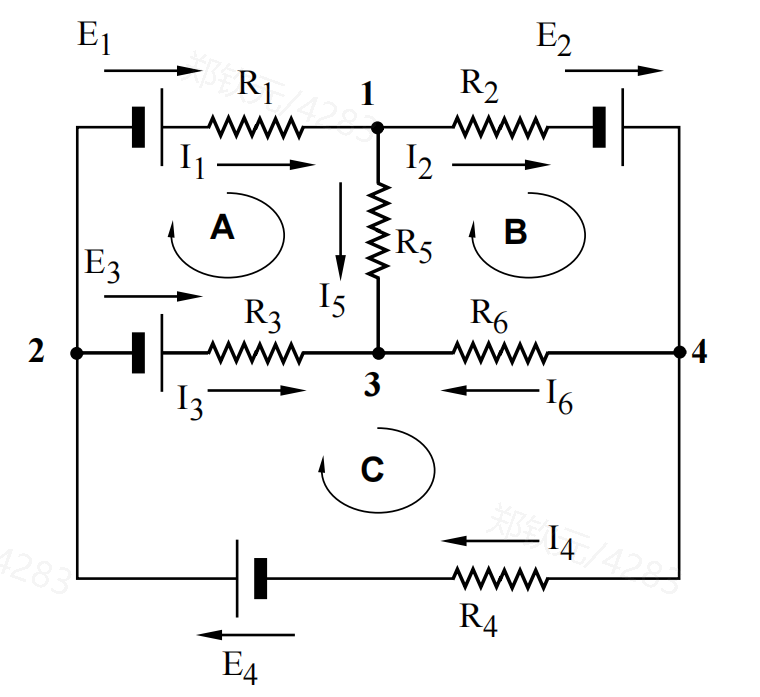
\includegraphics[width=\linewidth]{fig2.6.1} 
    \caption{图2.6.1}
    \label{fig:2.6.1}
\end{figure}

问题是将每个支路中的电流 \(I_k\) 与电阻 \(R_k\) 和电动势 \(E_k\) 联系起来。这可以通过使用欧姆定律结合基尔霍夫定律来产生线性方程组来实现。

\begin{bluebox}{欧姆定律}
欧姆定律指出:对于电流 \(I\) 安培,电阻 \(R\) 欧姆上的电压降(单位:伏特)为 \(V = IR\)。

对于大小为 \(E\) 的EMF源和电流 \(I\),源内部总是有一个小的内阻,其上的电压降为 \(V = E - I \times \text{内阻}\)。但内阻通常可忽略,因此源上的电压降可视为 \(V = E\)。当内阻不可忽略时,其效应可以合并到现有外部电阻中,或视为单独的外部电阻。
\end{bluebox}

\begin{bluebox}{基尔霍夫定律}
\textbf{节点规则:} 流向每个节点的电流的代数和为零。即,总流入电流必须等于总流出电流。这仅仅是电荷守恒的陈述。

\textbf{回路规则:} 每个回路中电动势的代数和必须等于同一回路中 \(IR\) 乘积的代数和。即,假设源内阻已考虑,则源上电压降的代数和等于每个回路中电阻上电压降的代数和。这是能量守恒的陈述。
\end{bluebox}

基尔霍夫定律可以在不知道电流和EMF方向的情况下使用。你可以任意指定方向。如果最终解中出现负值,则实际方向与假设方向相反。应用节点规则时,如果电流方向朝向节点,则视为正;否则视为负。显然,节点规则总是产生齐次方程组。例如,将节点规则应用于图2.6.1中的电路,会产生四个齐次方程,六个未知数(即 \(I_k\)):
\[
\begin{aligned}
&\text{节点1: } I_1 - I_2 - I_5 = 0 \\
&\text{节点2: } I_2 - I_3 - I_4 = 0 \\
&\text{节点3: } I_5 + I_6 - I_1 = 0 \\
&\text{节点4: } I_3 + I_4 - I_6 = 0
\end{aligned}
\]

应用回路规则时,必须选择某个方向(顺时针或逆时针)作为正方向,该方向上的所有EMF和电流视为正,相反方向视为负。一个电流在节点规则中可能被视为正,但在回路规则中使用时可能被视为负。如果正方向被视为顺时针,则将回路规则应用于图2.6.1中的三个指示回路A、B和C,会产生三个非齐次方程,六个未知数(\(I_k\) 视为未知数,而 \(R_k\) 和 \(E_k\) 假设已知):
\[
\begin{aligned}
&\text{回路A: } E_1 - E_2 = I_1 R_1 - I_2 R_2 \\
&\text{回路B: } E_2 = I_2 R_2 + I_3 R_3 + I_4 R_4 \\
&\text{回路C: } E_3 = I_4 R_4 - I_5 R_5 - I_6 R_6
\end{aligned}
\]

还有另外四个回路也会产生回路方程,总共有11个方程(4个节点方程和7个回路方程)和6个未知数。虽然这看起来是一个一般的 \(11 \times 6\) 方程组,但事实并非如此。如果电路处于平衡状态,则物理情况要求对于每组EMF \(E_k\),对应的电流 \(I_k\) 必须唯一确定。换句话说,物理保证由基尔霍夫定律产生的 \(11 \times 6\) 系统必须是一致的且具有唯一解。

假设 \([A \mid b]\) 表示由基尔霍夫定律生成的 \(11 \times 6\) 系统的增广矩阵。从 §2.5 的结果中,我们知道系统有唯一解当且仅当:
\[
\text{rank}(A) = \text{rank}([A \mid b]) = n = 6
\]
此外,§2.3 中证明了系统是一致的当且仅当:
\[
\text{rank}(A) = \text{rank}([A \mid b])
\]
结合这两个事实,我们可以得出结论:
\[
\text{rank}([A \mid b]) = \text{rank}(A) = 6
\]
因此,当 \([A \mid b]\) 被简化为 \(E_{[A \mid b]}\) 时,将恰好有6个非零行和5个零行。因此,原始11个方程中有5个是冗余的,因为它们可以通过特定6个“独立”方程的组合“归零”。最好提前知道11个方程中哪些是冗余的,哪些可以作为“独立”集。

注意,在使用节点规则时,节点4的方程仅仅是节点1、2和3方程的负和,且前三个方程是独立的,即三个方程中没有一个可以写为其他两个的组合。这种情况是典型的。对于具有 \(n\) 个节点的一般电路,可以证明前 \(n-1\) 个节点的方程是独立的,最后一个节点的方程是冗余的。

回路规则也会产生冗余方程。只有简单回路(不包含更小回路的回路)会产生独立方程。例如,考虑图2.6.1中由三个外部支路组成的大回路。将回路规则应用于这个大回路不会产生新信息,因为大回路可以通过“加”其内部的三个简单回路A、B和C来构造。与大外部回路相关的方程为:
\[
E_1 - E_2 + E_3 = I_1 R_1 - I_2 R_2 + I_3 R_3 + I_4 R_4 - I_5 R_5 - I_6 R_6
\]
这正好是对应三个组成回路A、B和C的方程之和。这种现象在一般情况下成立,因此使用回路规则时只需考虑简单回路。

讨论的要点是结论:更一般的 \(11 \times 6\) 矩形系统可以通过丢弃最后一个节点方程并仅使用简单回路方程,替换为等效的 \(6 \times 6\) 平方系统,该系统具有唯一解。这是实际工作的典型特征。问题的物理性质连同自然约束通常可用于将一般矩形系统替换为平方且具有唯一解的系统。

我们研究的目标之一是更清楚地理解此应用中出现的“独立性”概念。到目前为止,独立性是一个直观概念,但此示例有助于阐明独立性是一个基本重要概念,值得更牢固地确定。这将在§4.3中完成,并且从电路获得独立方程的一般理论在示例4.4.6和4.4.7中开发。

\textcolor{red}{练习2.6}
\color{red}\rule{\textwidth}{0.4pt}\color{black}

\begin{enumerate}[leftmargin=*, label=\bfseries 2.6.\arabic*]
    \item 假设在图2.6.1所示的电路中,\(R_i = i\) 欧姆,\(E_i = i\) 伏特。
    \begin{enumerate}[label=(\alph*)]
        \item 确定六个指示电流。
        \item 选择节点1作为参考点,并将其电位固定为0伏特。相对于此参考,计算其他三个节点的电位。通过验证每个回路的回路规则来检查你的答案。
    \end{enumerate}

    \item 确定以下电路中的三个指示电流。
    \begin{figure}[h]
        \centering
        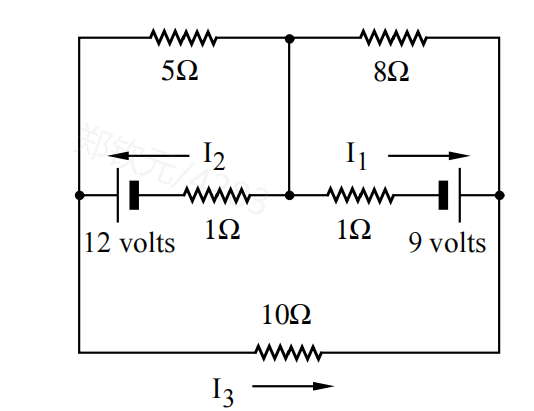
\includegraphics[width=\linewidth]{fig2.6.2} 
        \caption{图2.6.2}
        \label{fig:2.6.2}
    \end{figure}

    \item 确定以下电路中的两个未知EMF。
    \begin{figure}[h]
        \centering
        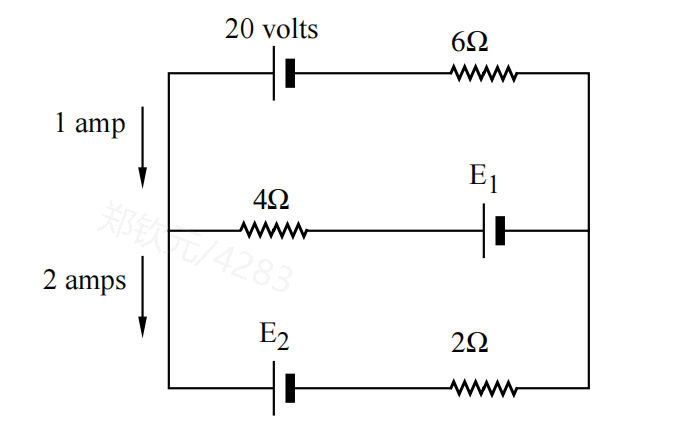
\includegraphics[width=\linewidth]{fig2.6.3} 
        \caption{图2.6.3}
        \label{fig:2.6.3}
    \end{figure}

    \item 考虑以下所示电路并回答以下问题。
    \begin{figure}[h]
        \centering
        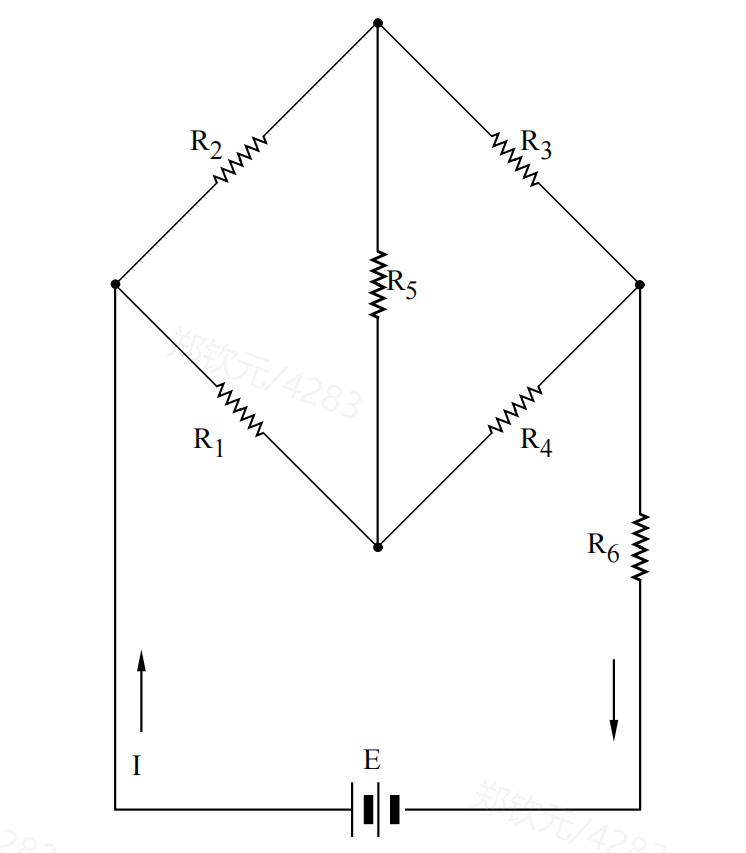
\includegraphics[width=\linewidth]{fig2.6.4} 
        \caption{图2.6.4}
        \label{fig:2.6.4}
    \end{figure}
    \begin{enumerate}[label=(\alph*)]
        \item 电路包含多少个节点?
        \item 电路包含多少个支路?
        \item 确定回路的总数,然后确定简单回路的数量。
        \item 证明简单回路方程形成“独立”方程组,即没有冗余方程。
        \item 验证任何三个节点方程构成“独立”方程组。
        \item 验证与包含 \(R_1, R_2, R_3, R_4\) 的回路相关的回路方程可以表示为包含在较大回路中的两个简单回路的两个方程之和。
        \item 如果 \(R_1 = R_2 = R_3 = R_4 = 1\) 欧姆,\(R_5 = R_6 = 5\) 欧姆,且 \(E = 5\) 伏特,确定指示电流 \(I\)。
    \end{enumerate}
\end{enumerate}


\section{矩阵系统与阶梯形}

% 定义画圈命令,用于标记主元
\newcommand{\circlednum}[1]{%
    \tikz[baseline=(char.base)]{%
        \node[draw, circle, inner sep=1pt] (char) {#1};%
    }%
}

\section{一般线性系统与阶梯形式}
正如我们在前一节中提到的,解线性方程组的方法是将其转化为增广矩阵,使用初等行变换将增广矩阵化简,然后解由简化矩阵表示的等价系统。这个过程如下图所示。

\begin{figure}[h]
    \centering
    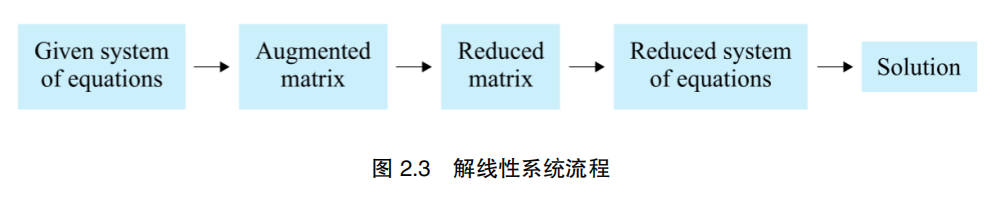
\includegraphics[width=\linewidth]{../images/2.1-1.png} % 请根据实际情况替换图片路径
    \caption{解线性系统流程}
    \label{fig:linear_system_process}
\end{figure}

我们了解了对于 \(n \times n\) 矩阵进行高斯消去的相关内容,这对应于有 \(n\) 个方程和 \(n\) 个未知数的情况。但是如果我们要推广到更一般的线性系统,该如何操作呢?在本节中,我们将介绍更一般的高斯消去法,给出一般线性系统矩阵的行阶梯形式。

我们的第一个目标是将高斯消元技术从方程组扩展到完全通用的矩形系统即线性系统方程的个数与变量的个数不相等的情况。回顾一下,对于具有唯一解的方程组,主元的位置总是位于系数矩阵 \(A\) 的主对角线上- 即从左上角到右下角的对角线上。这样做可以确保高斯消元导致 \(A\) 被减小为一个三角矩阵。以 \(n=4\) 为例,如下图所示:
\[
T=\begin{pmatrix} 
\circledast & * & * & * \\ 
0 & \circledast & * & * \\ 
0 & 0 & \circledast & * \\ 
0 & 0 & 0 & \circledast 
\end{pmatrix}
\]
我们知道主元必须是非零数。对于具有唯一解的方阵系统,我们总是可以在主对角线上的每个关键位置引入一个非零数。然而,在一般矩形系统的情况下,在系数矩阵中并不总是可能使主元位置位于一条直线上。这意味着高斯消去的最终结果不会是三角形的。例如,考虑以下系统:
\[
\begin{cases} 
x_{1}+2 x_{2}+x_{3}+3 x_{4}+3 x_{5}=5 \\ 
2 x_{1}+4 x_{2}+4 x_{4}+4 x_{5}=6 \\ 
x_{1}+2 x_{2}+3 x_{3}+5 x_{4}+5 x_{5}=9 \\ 
2 x_{1}+4 x_{2}+4 x_{4}+7 x_{5}=9 
\end{cases}
\]
该系统的系数矩阵为:
\[
A=\begin{pmatrix} 
1 & 2 & 1 & 3 & 3 \\ 
2 & 4 & 0 & 4 & 4 \\ 
1 & 2 & 3 & 5 & 5 \\ 
2 & 4 & 0 & 4 & 7 
\end{pmatrix}
\]
对系数矩阵 \(A\) 应用高斯消去法得到如下形式:
\[
\begin{pmatrix} 
\circlednum{1} & 2 & 1 & 3 & 3 \\ 
2 & 4 & 0 & 4 & 4 \\ 
1 & 2 & 3 & 5 & 5 \\ 
2 & 4 & 0 & 4 & 7 
\end{pmatrix}
\to
\begin{pmatrix} 
1 & 2 & 1 & 3 & 3 \\ 
0 & \circlednum{0} & -2 & -2 & -2 \\ 
0 & 0 & 2 & 2 & 2 \\ 
0 & 0 & -2 & -2 & 1 
\end{pmatrix}
\]
在之前所讨论的高斯消去的过程中,从第一行开始向下然后向右进行消除,如果向右移动下一个位置进行消除时,此时该位置元素为0,这时则执行与该位置所在行以下的行的交换,以便将非零数带入该位置。但是,在本例中,显然不可能通过将第二行与较低的行互换来将非零数带入 \((2,2)\) 位置。

\subsection{高斯消去法的改进与行阶梯型(Row Echelon Form)}
我们知道在一般矩形系统的情况下,对系数矩阵作高斯消去时在矩阵中并不总是可能使主元位置位于一条对角直线上。这意味着高斯消去的最终结果不会是三角形式。为了处理这种情况,我们对高斯消去做了一定的修改。

\begin{bluebox}{修正后的高斯消元法}
假设 \(U\) 是第 \(i-1\) 步高斯消去后的系统增广矩阵。执行第 \(i\) 步的步骤如下:
\begin{itemize}
    \item 在 \(U\) 中从左到右移动,找到第 \(i\) 个非零位置或该位置下面包含非零元素的那一列,我们把这一列写作 \(U_{* j}\)。
    \item 第 \(i\) 步高斯消去后的主元位置是在 \((i, j)\)。
    \item 如果 \((i, j)\) 的元素为0,则可以将第 \(i\) 行与下面的非零行交换,将一个非零数带入 \((i, j)\) 位置,然后消去这个主元以下的所有元素。
    \item 如果行 \(U_{i *}\) 以及下面 \(U\) 中的所有行都是零,那么消除过程就完成了。
\end{itemize}
\end{bluebox}

% 红色文字
\textcolor{red}{例子2.1.1}
% 红色水平线(宽度为文本宽度,厚度0.4pt)
\color{red}\rule{\textwidth}{0.4pt}\color{black}

对以下矩阵应用修正高斯消去法,圈出支点位置:
\[
A=\begin{pmatrix} 
1 & 2 & 1 & 3 & 3 \\ 
2 & 4 & 0 & 4 & 4 \\ 
1 & 2 & 3 & 5 & 5 \\ 
2 & 4 & 0 & 4 & 7 
\end{pmatrix}
\]
解答:
\[
\begin{pmatrix} 
\circlednum{1} & 2 & 1 & 3 & 3 \\ 
2 & 4 & 0 & 4 & 4 \\ 
1 & 2 & 3 & 5 & 5 \\ 
2 & 4 & 0 & 4 & 7 
\end{pmatrix}
\to
\begin{pmatrix} 
\circlednum{1} & 2 & 1 & 3 & 3 \\ 
0 & 0 & \circlednum{2} & -2 & -2 \\ 
0 & 0 & 2 & 2 & 2 \\ 
0 & 0 & -2 & -2 & 1 
\end{pmatrix}
\]

\[
\to
\begin{pmatrix} 
\circlednum{1} & 2 & 1 & 3 & 3 \\ 
0 & 0 & \circlednum{2} & -2 & -2 \\ 
0 & 0 & 0 & 0 & \circlednum{0} \\ 
0 & 0 & 0 & 0 & 3 
\end{pmatrix}
\to
\begin{pmatrix} 
\circlednum{1} & 2 & 1 & 3 & 3 \\ 
0 & 0 & \circlednum{2} & -2 & -2 \\ 
0 & 0 & 0 & 0 & \circlednum{3} \\ 
0 & 0 & 0 & 0 & 0 
\end{pmatrix}
\]
上面的例子中应用高斯消去的最终结果不是一个纯粹的三角形形式,而是一个锯齿状或"阶梯"类型的三角形形式。此后,具有这种阶梯结构的矩阵将被称为行阶梯形式。

\begin{bluebox}{修正后的高斯消元法}
一个 \(m \times n\) 矩阵 \(E\),其行 \(E_{i *}\),列 \(E_{* j}\) 被称为行阶梯形,满足下面两个条件:
\begin{itemize}
    \item 如果 \(E_{i *}\) 全部由0组成,那么 \(E_{i}\) 下面的所有行也全部为0,即所有的零行都在 \(E\) 底部。
    \item 如果 \(E_{i}\) 中的第一个非零项在第 \(j\) 个位置,那么在这之前的所有列在 \(E_{* 1}, E_{* 2}, \cdots, E_{* j}\) 中第 \(i\) 行位置以下的项全为0。
\end{itemize}
\end{bluebox}

这两个条件说明,行阶梯形中的非零元素必须位于或高于一条阶梯线,这条线从左上角开始,并向右向下倾斜。主元是每一行的第一个非零项。行阶梯形矩阵的典型结构如下图所示:
\[
\begin{pmatrix} 
\circledast & * & * & * & * & * & * & * \\ 
0 & 0 & \circledast & * & * & * & * & * \\ 
0 & 0 & 0 & \circledast & * & * & * & * \\ 
0 & 0 & 0 & 0 & 0 & 0 & \circledast & * \\ 
0 & 0 & 0 & 0 & 0 & 0 & 0 & 0 \\ 
0 & 0 & 0 & 0 & 0 & 0 & 0 & 0 
\end{pmatrix}
\]
由于选择行变换将矩阵 \(A\) 简化为行阶梯形 \(E\) 的灵活性, \(E\) 中的元素不是唯一由 \(A\) 决定的。但是,可以证明 \(E\) 的"形式"是唯一的,因为 \(E(A)\) 中的主元位置是唯一由矩阵 \(A\) 中的元素决定的。因此,主元的个数与 \(E\) 中的非零行数相同,它唯一由 \(A\) 中的元素确定。主元的个数通常成为矩阵 \(A\) 的秩。它在矩阵分析中起到至关重要的作用。

\begin{bluebox}{矩阵的秩(Rank of a Matrix)}
假设矩阵 \(A_{m \times n}\) 通过行变换化为阶梯形 \(E\), 那么矩阵 \(A\) 的秩被定义为下面这个数:
\[
\begin{aligned} 
rank(A) & = \text{矩阵中主元的数量} \\ 
& = \text{矩阵 E 中非零行的数量} \\ 
& = \text{矩阵 A 中的基本列的数量} 
\end{aligned}
\]
其中矩阵 \(A\) 的基本列被定义为 \(A\) 中包含主元位置的列。
\end{bluebox}
 
% 红色文字
\textcolor{red}{例子 2.1.2}
% 红色水平线(宽度为文本宽度,厚度0.4pt)
\color{red}\rule{\textwidth}{0.4pt}\color{black}

Problem: Determine the rank, and identify the basic columns in
\[
A = 
\begin{pmatrix}
1 & 2 & 1 & 1 \\
2 & 4 & 2 & 2 \\
3 & 6 & 3 & 4
\end{pmatrix}
\]

\textbf{Solution:} Reduce \( A \) to row echelon form as shown below:

\[
A = 
\begin{pmatrix}
1 & 2 & 1 & 1 \\
2 & 4 & 2 & 2 \\
3 & 6 & 3 & 4
\end{pmatrix}
\rightarrow
\begin{pmatrix}
1 & 2 & 1 & 1 \\
0 & 0 & 0 & 0 \\
0 & 0 & 0 & 1
\end{pmatrix}
\rightarrow
\begin{pmatrix}
1 & 2 & 1 & 1 \\
0 & 0 & 0 & 1 \\
0 & 0 & 0 & 0
\end{pmatrix}
= E
\]

Consequently, \( \text{rank}(A) = 2 \). The pivotal positions lie in the first and fourth columns so that the basic columns of \( A \) are \( A_{*1} \) and \( A_{*4} \). That is,

\[
\text{Basic Columns} = 
\left\{ 
\begin{pmatrix}
1 \\
2 \\
3
\end{pmatrix},
\begin{pmatrix}
1 \\
2 \\
4
\end{pmatrix}
\right\}
\]

Pay particular attention to the fact that the basic columns are extracted from \( A \) and not from the row echelon form \( E \).

\[
\begin{array}{c}
\text{pivot} \\
\downarrow \\
\begin{pmatrix}
1 & 4 & 5 & -9 & -7 \\
-1 & -2 & -1 & 3 & 1 \\
-2 & -3 & 0 & 3 & -1 \\
0 & -3 & -6 & 4 & 9
\end{pmatrix}\\
\uparrow \text{pivot column}
\end{array}
\]

% 红色文字
\textcolor{red}{练习2.1, 可以参考 ccjou.wordpress.com/2015/03/02/可对角化矩阵的分解篇/ Page 26}
% 红色水平线(宽度为文本宽度,厚度0.4pt)
\color{red}\rule{\textwidth}{0.4pt}\color{black}

\begin{enumerate}[leftmargin=*, label=\bfseries 2.1.\arabic*]

\item Reduce each of the following matrices to row echelon form, determine the rank, and identify the basic columns.

\begin{enumerate}[label=(\alph*)]
    \item $\begin{pmatrix}
        1 & 2 & 3 & 3 \\
        2 & 4 & 6 & 9 \\
        2 & 6 & 7 & 6
    \end{pmatrix}$
    
    \item $\begin{pmatrix}
        1 & 2 & 3 \\
        2 & 6 & 8 \\
        2 & 6 & 0 \\
        1 & 2 & 5 \\
        3 & 8 & 6
    \end{pmatrix}$
    
    \item $\begin{pmatrix}
        2 & 1 & 1 & 3 & 0 & 4 & 1 \\
        4 & 2 & 4 & 4 & 1 & 5 & 5 \\
        2 & 1 & 3 & 1 & 0 & 4 & 3 \\
        6 & 3 & 4 & 8 & 1 & 9 & 5 \\
        0 & 0 & 3 & -3 & 0 & 0 & 3 \\
        8 & 4 & 2 & 14 & 1 & 13 & 3
    \end{pmatrix}$
\end{enumerate}

\item Determine which of the following matrices are in row echelon form:

\begin{enumerate}[label=(\alph*)]
    \item $\begin{pmatrix}
        1 & 2 & 3 \\
        0 & 0 & 4 \\
        0 & 1 & 0
    \end{pmatrix}$
    
    \item $\begin{pmatrix}
        0 & 0 & 0 & 0 \\
        0 & 1 & 0 & 0 \\
        0 & 0 & 0 & 1
    \end{pmatrix}$
    
    \item $\begin{pmatrix}
        2 & 2 & 3 & -4 \\
        0 & 0 & 7 & -8 \\
        0 & 0 & 0 & -1
    \end{pmatrix}$
    
    \item $\begin{pmatrix}
        1 & 2 & 0 & 0 & 1 & 0 \\
        0 & 0 & 0 & 1 & 0 & 0 \\
        0 & 0 & 0 & 0 & 0 & 1 \\
        0 & 0 & 0 & 0 & 0 & 0
    \end{pmatrix}$
\end{enumerate}

\item Suppose that \( A \) is an \( m \times n \) matrix. Give a short explanation of why each of the following statements is true.

\begin{enumerate}[label=(\alph*)]
    \item \(\text{rank}(A) \leq \min\{m, n\}\).
    
    \item \(\text{rank}(A) < m\) if one row in \( A \) is entirely zero.
    
    \item \(\text{rank}(A) < m\) if one row in \( A \) is a multiple of another row.
    
    \item \(\text{rank}(A) < m\) if one row in \( A \) is a combination of other rows.
    
    \item \(\text{rank}(A) < n\) if one column in \( A \) is entirely zero.
\end{enumerate}

\item Let \( A = \begin{pmatrix}
    .1 & .2 & .3 \\
    .4 & .5 & .6 \\
    .7 & .8 & .901
\end{pmatrix} \).

\begin{enumerate}[label=(\alph*)]
    \item Use exact arithmetic to determine \(\text{rank}(A)\).
    
    \item Now use 3-digit floating-point arithmetic (without partial pivoting or scaling) to determine \(\text{rank}(A)\). This number might be called the "3-digit numerical rank."
    
    \item What happens if partial pivoting is incorporated?
\end{enumerate}

\item How many different "forms" are possible for a \( 3 \times 4 \) matrix that is in row echelon form?

\item Suppose that \([A | b]\) is reduced to a matrix \([E | c]\).

\begin{enumerate}[label=(\alph*)]
    \item Is \([E | c]\) in row echelon form if \( E \) is?
    
    \item If \([E | c]\) is in row echelon form, must \( E \) be in row echelon form?
\end{enumerate}

\end{enumerate}



% XeLatex编辑

\begin{document}

% \ucascover

% % --- 目录 ---
% % 会自动生成带“目录”标题的目录页
% \tableofcontents
% \newpage

% % --- 正文开始 ---


\subsection*{2.2 行简化阶梯形矩阵(REDUCED ROW ECHELON FORM)}

在 2.1 节中,我们引入了行阶梯形的概念。若在高斯-约当消元法的基础上再施加两个额外的条件,我们将得到一种形式更简洁、性质更优良的矩阵,称为\textbf{行简化阶梯形矩阵}。

\subsubsection*{2.2.1行简化阶梯形的定义}

一个 \( m \times n \) 的矩阵 \( E \) 被称为是\textbf{行简化阶梯形},当且仅当它满足以下三个条件:
\begin{enumerate}
    \item \( E \) 是行阶梯形矩阵。
    \item \textbf{每个主元(即每行第一个非零元素)均为 1}。
    \item \textbf{每个主元所在的列中,除主元自身外,其他所有元素均为 0}。
\end{enumerate}

行简化阶梯形矩阵的典型结构如下所示,其中标有 \(*\) 的元素可以是任意数(零或非零):

\[
E = \begin{pmatrix}
1 & * & 0 & 0 & * & * & 0 & * \\
0 & 0 & 1 & 0 & * & * & 0 & * \\
0 & 0 & 0 & 1 & * & * & 0 & * \\
0 & 0 & 0 & 0 & 0 & 0 & 1 & * \\
0 & 0 & 0 & 0 & 0 & 0 & 0 & 0 \\
0 & 0 & 0 & 0 & 0 & 0 & 0 & 0
\end{pmatrix}
\]

\subsubsection*{2.2.2行简化阶梯形的唯一性}

行简化阶梯形一个至关重要的性质是其\textbf{唯一性}。
\begin{itemize}
    \item 对于任意矩阵 \( A \),无论采用何种初等行变换序列将其化简,最终得到的行简化阶梯形矩阵 \( E_A \) 都是\textbf{唯一确定}的。
    \item 这种唯一性使得 \( E_A \) 在理论分析中非常有用,它可以作为一个"地图"或"密钥",来揭示原始矩阵 \( A \) 的列向量之间隐藏的线性关系。
\end{itemize}

\subsubsection*{2.2.3列关系在 \( E_A \) 与 \( A \) 中的体现}

在简化形式 \( E_A \) 中,列向量之间的关系是清晰透明的:
\begin{itemize}
    \item 每一个非基本列 \( E_{*k} \) 都可以表示为位于其左侧的基本列 \( E_{*b_1}, E_{*b_2}, \dots, E_{*b_j} \) 的线性组合:
    \[
    E_{*k} = \mu_1 E_{*b_1} + \mu_2 E_{*b_2} + \cdots + \mu_j E_{*b_j}
    \]
    其中,系数 \( \mu_1, \mu_2, \dots, \mu_j \) 恰好就是向量 \( E_{*k} \) 中的前 \( j \) 个分量。
    
    \item \textbf{关键洞察}:存在于 \( E_A \) 的列之间的这种线性依赖关系,与原始矩阵 \( A \) 的列之间的依赖关系\textbf{完全一致}。因此,若在 \( E_A \) 中有:
    \[
    E_{*k} = \mu_1 E_{*b_1} + \mu_2 E_{*b_2} + \cdots + \mu_j E_{*b_j}
    \]
    那么在 \( A \) 中,必然有:
    \[
    A_{*k} = \mu_1 A_{*b_1} + \mu_2 A_{*b_2} + \cdots + \mu_j A_{*b_j}
    \]
\end{itemize}

% 红色文字
\textcolor{red}{例子2.2.1}
% 红色水平线(宽度为文本宽度,厚度0.4pt)
\color{red}\rule{\textwidth}{0.4pt}\color{black}\\
将矩阵 \( A \) 的每个非基本列表示为基本列的线性组合。
\[
A = \begin{pmatrix}
2 & -4 & -8 & 6 & 3 \\
0 & 1 & 3 & 2 & 3 \\
3 & -2 & 0 & 0 & 8
\end{pmatrix}
\]

解答:
通过初等行变换将 \( A \) 化为行简化阶梯形 \( E_A \):
\[
\begin{pmatrix}
2 & -4 & -8 & 6 & 3 \\
0 & 1 & 3 & 2 & 3 \\
3 & -2 & 0 & 0 & 8
\end{pmatrix}
\rightarrow \cdots \rightarrow
\begin{pmatrix}
1 & 0 & 2 & 0 & 4 \\
0 & 1 & 3 & 0 & 2 \\
0 & 0 & 0 & 1 & \frac{1}{2}
\end{pmatrix} = E_A
\]

在 \( E_A \) 中,第 1, 2, 4 列是基本列。观察非基本列:
\begin{itemize}
    \item \( E_{*3} = 2E_{*1} + 3E_{*2} \)
    \item \( E_{*5} = 4E_{*1} + 2E_{*2} + \frac{1}{2}E_{*4} \)
\end{itemize}

因此,在原始矩阵 \( A \) 中,同样的关系成立:
\begin{itemize}
    \item \( A_{*3} = 2A_{*1} + 3A_{*2} \)
    \item \( A_{*5} = 4A_{*1} + 2A_{*2} + \frac{1}{2}A_{*4} \)
\end{itemize}

可以通过直接计算验证这些等式的正确性。

总结:行简化阶梯形 \( E_A \) 的效用在于它能清晰地揭示出以矩阵列形式存储的数据之间的内在依赖关系,这是普通行阶梯形所不具备的强大理论工具。

% 红色文字
\textcolor{red}{练习2.2}
% 红色水平线(宽度为文本宽度,厚度0.4pt)
\color{red}\rule{\textwidth}{0.4pt}\color{black}

\begin{enumerate}[leftmargin=*, label=\bfseries 2.2.\arabic*]

\item Determine the reduced row echelon form for each of the following matrices and then express each nonbasic column in terms of the basic columns:
\begin{enumerate}[label=(\alph*)]
    \item \(\begin{pmatrix}
        1 & 2 & 3 & 3 \\
        2 & 4 & 6 & 9 \\
        2 & 6 & 7 & 6 
    \end{pmatrix}\)
    
    \item \(\begin{pmatrix}
        2 & 1 & 1 & 3 & 0 & 4 & 1 \\
        4 & 2 & 4 & 4 & 1 & 5 & 5 \\
        2 & 1 & 3 & 1 & 0 & 4 & 3 \\
        6 & 3 & 4 & 8 & 1 & 9 & 5 \\
        0 & 0 & 3 & -3 & 0 & 0 & 3 \\
        8 & 4 & 2 & 14 & 1 & 13 & 3 
    \end{pmatrix}\)
\end{enumerate}

\item Construct a matrix \( A \) whose reduced row echelon form is
\[
E_A = \begin{pmatrix}
1 & 2 & 0 & -3 & 0 & 0 & 0 \\
0 & 0 & 1 & -4 & 0 & 1 & 0 \\
0 & 0 & 0 & 0 & 1 & 0 & 0 \\
0 & 0 & 0 & 0 & 0 & 0 & 1 \\
0 & 0 & 0 & 0 & 0 & 0 & 0 \\
0 & 0 & 0 & 0 & 0 & 0 & 0 
\end{pmatrix}.
\]
Is \( A \) unique?

\item Suppose that \( A \) is an \( m \times n \) matrix. Give a short explanation of why \( \text{rank}(A) < n \) whenever one column in \( A \) is a combination of other columns in \( A \).

\item Consider the following matrix:
\[
A = \begin{pmatrix}
.1 & .2 & .3 \\
.4 & .5 & .6 \\
.7 & .8 & .901 
\end{pmatrix}.
\]
\begin{enumerate}[label=(\alph*)]
    \item Use exact arithmetic to determine \( E_A \).
    \item Now use 3-digit floating-point arithmetic (without partial pivoting or scaling) to determine \( E_A \) and formulate a statement concerning "near relationships" between the columns of \( A \).
\end{enumerate}

\item Consider the matrix
\[
E = \begin{pmatrix}
1 & 0 & -1 \\
0 & 1 & 2 \\
0 & 0 & 0 
\end{pmatrix}.
\]
You already know that \( E_{*3} \) can be expressed in terms of \( E_{*1} \) and \( E_{*2} \). However, this is not the only way to represent the column dependencies in \( E \). Show how to write \( E_{*1} \) in terms of \( E_{*2} \) and \( E_{*3} \) and then express \( E_{*2} \) as a combination of \( E_{*1} \) and \( E_{*3} \).

\noindent \textbf{Note:} This exercise illustrates that the set of pivotal columns is not the only set that can play the role of "basic columns." Taking the basic columns to be the ones containing the pivots is a matter of convenience because everything becomes automatic that way.

\end{enumerate}

\end{document}


\subsection*{2.3 线性方程组的一致性(Consistency Of Linear Systems)}

如果一个包含 \(n\) 个未知数的 \(m\) 个线性方程组至少有一个解,则称其为相容方程组。如果没有解,则该方程组
被称为不相容方程组。本节旨在确定给定方程组相容的条件。

对于仅包含两个或三个未知数的方程组,
说明其相容性条件很容易。两个未知数的线性方程表示二维空间中的一条直线,
而三个未知数的线性方程表示三维空间中的平面。因此,
一个包含 \(m\) 个两个未知数的线性方程组相容当且仅当这 \(m\) 个方程定义的 \(m\) 条直线至少有一个公共交点。
同样,一个包含 \(m\) 个三个未知数的方程组相容当且仅当
相关的 \(m\) 个平面至少有一个公共交点。
然而,当 \(m\) 较大时,这些几何条件可能不易直观验证,而当 \(n\) > 3 时,相交线或平面的推广则无法用肉眼直观地看到。

我们不依赖几何来建立一致性,而是使用高斯消元法。如果将相关的增广矩阵 \([A|b]\) 通过行运算简化为行阶梯矩阵 \([E|c]\),则一致性(或不一致性)变得显而易见。
假设在将 \([A|b]\) 简化为 \([E|c]\) 的过程中,出现这样一种情况:一行中唯一的非零项出现在右侧,如下所示:

\[
\mathrm{Row}\_i \rightarrow 
\left(\begin{array}{cccccc|c}
* & * & * & * & * & * & * \\ 
0 & 0 & 0 & * & * & * & * \\ 
0 & 0 & 0 & 0 & 0 & 0 & \alpha \\
\bullet & \bullet & \bullet & \bullet & \bullet & \bullet & \bullet \\
\bullet & \bullet & \bullet & \bullet & \bullet & \bullet & \bullet \\
\end{array}\right)
\leftarrow \alpha \neq 0.
\]

如果这发生在第 i 行,则相关系统的第 i 个方程为

\[
0x_1 + 0x_2 + ... + 0x_n = \alpha.
\]

当 \(\alpha \neq 0\) 时,该方程无解,因此原系统也必然不一致(因为行运算不会改变解集)。
反之亦然。也就是说,如果一个系统不一致,那么在消元过程中,会出现如下形式的行

\[
\left(\begin{array}{cccccc|c}
0 & 0 & ... & 0 & \alpha
\end{array}\right), \alpha \neq 0.
\]

否则,回代过程可以完成,并产生一个解。当遇到形式为
(0 0 ... 0 \(\mid\) 0) 的行时,不会指示不一致性。这只是表示 0 = 0,
尽管这对于确定任何未知数的值没有任何帮助,但它仍然是一个真实的陈述,
因此它并不表示系统存在不一致。

还有一些其他方法可以表征系统的一致性(或不一致性)。其中一种方法是:如果增广矩阵 \([A|b]\) 的最后一列 \(b\) 是非基列,则最后一列不可能存在主元,因此系统是一致的,因为 (2.3.1) 的情况不会发生。
反之,如果系统是一致的,那么 (2.3.1) 的情况在高斯消元法中永远不会发生,因此最后一列不可能是基列。换句话说,\([A|b]\) 是一致的当且仅当 \(b\) 是非基列。

说 b 是 \([A|b]\) 中的非基列,等同于说\([A|b]\) 中的所有基列都位于系数矩阵 A 中。由于矩阵中基列的数量就是秩,因此一致性也可以这样来描述:
当且仅当 rank\([A|b]\) = rank\((A)\) 时,系统才是一致的。



\begin{bluebox}{线性方程组的一致性}
满足以下任意一个条件都可以说 \([A|b]\) 是一致的:
\begin{itemize}
    \item 行简化阶梯形矩阵 \([A|b]\) 中不存在形如下列的行:
    \[
    \left(\begin{array}{cccc|c}
        0 & 0 & ... & 0 & \alpha
    \end{array}\right), \alpha \neq 0
    \]
    \item \(b\) 是 \([A|b]\) 中的非基列。
    \item rank\([A|b]\) = rank\((A)\)
    \item \(b\) 是 \(A\) 的基列的一个组合。
\end{itemize}
\end{bluebox}

% 红色文字
\textcolor{red}{例子2.3.1}
% 红色水平线(宽度为文本宽度,厚度0.4pt)
\color{red}\rule{\textwidth}{0.4pt}\color{black}

\textbf{问题}: 确定以下系统是否一致: 
\[
\begin{align} 
    x_1 + x_2 + 2x_3 + 2x_4 + x_5 = 1, \\
    2x_1 + 2x_2 + 4x_3 + 4x_4 + 3x_5 = 1, \\
    2x_1 + 2x_2 + 4x_3 + 4x_4 + 2x_5 = 2, \\
    3x_1 + 5x_2 + 8x_3 + 6x_4 + 5x_5 = 3.
\end{align}
\]
\textbf{解答}: 对增广矩阵 \([A|b]\) 应用高斯消元法,如下所示
\[
\left(\begin{array}{ccccc|c} 
\circlednum{1} & 1 & 2 & 2 & 1 & 1 \\ 
2 & 2 & 4 & 4 & 3 & 1 \\ 
2 & 2 & 4 & 4 & 2 & 2 \\ 
3 & 5 & 8 & 6 & 5 & 3 
\end{array}\right)
\to
\left(\begin{array} {ccccc|c} 
\circlednum{1} & 1 & 2 & 2 & 1 & 1 \\ 
0 & \circlednum{0} & 0 & 0 & 1 & -1 \\ 
0 & 0 & 0 & 0 & 0 & 0 \\ 
0 & 2 & 2 & 0 & 2 & 0 
\end{array}\right)
\to
\left(\begin{array}{ccccc|c} 
\circlednum{1} & 1 & 2 & 2 & 1 & 1 \\ 
0 & \circlednum{2} & 2 & 0 & 2 & 0 \\ 
0 & 0 & 0 & 0 & \circlednum{1} & -1 \\ 
0 & 0 & 0 & 0 & 0 & 0 
\end{array}\right)
\]

由于形式为 \left(\begin{array}{cccc|c} 0 & 0 & ... & 0 & \alpha \end{array}\right), 
\(\alpha \neq 0\) 的行从未出现,
因此系统是一致的。我们还可以观察到,\(b\) 是 \([A|b]\) 中的非基本列,
因此 rank\([A|b]\) = rank \((A)\)。最后,通过将 \(A\) 完全约化为
\(E_A\),可以验证 \(b\) 确实是基本列的组合,\{\(A_{*1}, A_{*2}, A_{*5}\)\}。

% 红色文字
\textcolor{red}{练习 2.3}
% 红色水平线(宽度为文本宽度,厚度0.4pt)
\color{red}\rule{\textwidth}{0.4pt}\color{black}

\begin{enumerate}[leftmargin=*, label=\bfseries 2.3.\arabic*]

\item Determine which of the following systems are consistent.

\begin{enumerate}[label=(\alph*)]
    \item \(\begin{array}{l}
    x + 2y + z = 2, \\
    2x + 4y = 4, \\
    3x + 6y + z = 4.
    \end{array}\)
    
    \item \(\begin{array}{l}
    2x + 2y + 4z = 0, \\
    3x + 2y + 5z = 0, \\
    4x + 2y + 6z = 0.
    \end{array}\)
    
    \item \(\begin{array}{l}
    x - y + z = 1, \\
    x - y - z = 2, \\
    x + y - z = 3, \\
    x + y + z = 4.
    \end{array}\)

    \item \(\begin{array}{l}
    x - y + z = 1, \\
    x - y - z = 2, \\
    x + y - z = 3, \\
    x + y + z = 2.
    \end{array}\)

    \item \(\begin{array}{l}
    2w + x + 3y + 5z = 1, \\
    4w + 4y + 8z = 0, \\
    w + x + 2y + 3z = 0, \\
    x + y + z = 0.
    \end{array}\)

    \item \(\begin{array}{l}
    2w + x + 3y + 5z = 7, \\
    4w + 4y + 8z = 8, \\
    w + x + 2y + 3z = 5, \\
    x + y + z = 3.
    \end{array}\)
\end{enumerate}

\item Construct a \(3 \times 4\) matrix \(A\) and \(3 \times 1\) columns \(b\) and \(c\) such that \([A|b]\) is the augmented matrix for an inconsistent system, but \([A|c]\) is the augmented matrix for a consistent system.

\item If \(A\) is an \(m \times n\) matrix with rank\((A) = m\), explain why the system \([A|b]\) must be consistent for every right-hand side \(b\).

\item Is it possible for a parabola whose equation has the form \(y = \alpha+\beta x+\gamma x^2\) to pass through the four points (0, 1), (1, 3), (2, 15), and (3, 37)? Why?

\item Consider using floating-point arithmetic (without scaling) to solve the following system:
\[
\begin{array}{l}
.835x + .667y = .168, \\
.333x + .266y = .067.
\end{array}
\]
\begin{enumerate}[label=(\alph*)]
    \item Is the system consistent when 5-digit arithmetic is used?
    
    \item What happens when 6-digit arithmetic is used?
\end{enumerate}

\item In order to grow a certain crop, it is recommended that each square foot of ground be treated with 10 units of phosphorous, 9 units of potassium, and 19 units of nitrogen. 
Suppose that there are three brands of fertilizer on the market— say brand \(\mathcal{X}\) , brand \(\mathcal{Y}\) , and brand \(\mathcal{Z}\).
One pound of brand \(\mathcal{X}\) contains 2 units of phosphorous, 3 units of potassium, and 5 units of nitrogen. One pound of brand \(\mathcal{Y}\) contains 1 unit of phosphorous,
3 units of potassium, and 4 units of nitrogen. One pound of brand \(\mathcal{Z}\) contains only 1 unit of phosphorous and 1 unit of nitrogen.
Determine whether or not it is possible to meet exactly the recommendation by applying some combination of the three brands of fertilizer.

\item Suppose that an augmented matrix \([A|b]\) is reduced by means of Gaussian elimination to a row echelon form \([E|c]\). If a row of the form 
\[
\left(\begin{array}{cccc|c}
    0 & 0 & ... & 0 & \alpha
\end{array}\right), \alpha \neq 0
\]
does not appear in \([E|c]\), is it possible that rows of this form could have appeared at earlier stages in the reduction process? Why?

\end{enumerate}

\subsection*{2.4 齐次系统(Homogeneous Systems)}

\(n\) 个未知数的 \(m\) 个线性方程组
\[
\begin{array}{cols}
    a_{11}x_1 + a_{12}x_2 + ... + a_{1n}x_n = 0, \\
    a_{21}x_1 + a_{22}x_2 + ... + a_{2n}x_n = 0, \\
    \vdots \\
    a_{m1}x_1 + a_{m2}x_2 + ... + a_{mn}x_n = 0.
\end{array}
\]

如果方程式的右侧完全由0组成,则称其为\textbf{齐次系统}。如果方程式的右侧至少有一个非零数,则该系统称为\textbf{非齐次系统}。本节旨在探讨齐次系统的一些基本概念。

在处理齐次方程组时,一致性从来都不是问题,因为无论系数值如何,
零解 \(x_1 = x_2 = ... = x_n = 0\) 始终是唯一解。下文中,
将全零组成的解称为\textbf{平凡解}。唯一的问题是:“除了平凡解之外,还有其他解吗?
如果有,我们如何才能最好地描述它们?” 和之前一样,高斯消元法可以给出答案。

使用高斯消元法将齐次系统的增广矩阵 \([A|0]\) 化简为行阶梯形时,右侧的零列不会被任何三种基本行运算改变。
也就是说,任何通过行运算从 \([A|0]\) 导出的行阶梯形,也必然具有 \([E|0]\) 的形式。这意味着最后一列的零只是
多余的负担,没有必要在每一步都带上去。只需将系数矩阵 \(A\) 化简为行阶梯形 \(E\),并记住在执行回代时,右侧
完全为零。通过一个典型的例子,可以更好地理解这个过程。

为了求解齐次系统的解
\[
\begin{array}{cols}
    x_1 + 2x_2 + 2x_3 + 3x_4 = 0, \\
    2x_1 + 4x_2 + x_3 + 3x_4 = 0, \\
    3x_1 + 6x_2 + x_3 + 4x_4 = 0,
\end{array}
\]
将系数矩阵简化为行阶梯形式。
\[
A = 
\left(\begin{array}{cccc}
1 & 2 & 2 & 3 \\
2 & 4 & 1 & 3 \\
3 & 6 & 1 & 4
\end{array}\right)\to
\left(\begin{array}{cccc}
1 & 2 & 2 & 3 \\
0 & 0 & -3 & -3 \\
0 & 0 & -5 & -5
\end{array}\right)\to
\left(\begin{array}{cccc}
1 & 2 & 2 & 3 \\
0 & 0 & -3 & -3 \\
0 & 0 & 0 & 0
\end{array}\right)
= E
\]
因此,原始齐次系统等价于以下简化齐次系统:
\[
\begin{array}{cols}
    x_1 + 2x_2 + 2x_3 + 3x_4 = 0, \\
    -3x_3 - 3x_4 = 0.
\end{array}
\]
由于这个简化系统中有四个未知数,但只有两个方程,因此不可能为每个未知数求出唯一的解。我们能做的最好的事情是,
选择两个“基本”未知数——我们称之为\textbf{基本变量},并用另外两个未知数来求解它们——这两个未知数的值必须
保持任意或“自由”,因此它们被称为\textbf{自由变量}。虽然选择一组基本变量有多种可能性,但惯例是始终求解与枢轴位置对应的未知数,
或者,等价地,与基本列对应的未知数。在这个例子中,枢轴(以及基本列)位于第一和第三位置,
因此策略是应用回代法,用自由变量 \(x_2\) 和 \(x_4\) 来求解简化系统中的基本变量 \(x_1\) 和 \(x_3\)。由第二个方程得出
\[
x_3 = -x_4.
\]
代入第一个方程可得
\[
\begin{align}
x_1 &= -2x_2 -2x_3 - 3x_4, \\
&= -2x_2 - 2(-x_4) - 3x_4, \\
&= -2x_2 - x_4.
\end{align}
\]
因此,原齐次系统的所有解都可以描述为
\[
\begin{align}
    &x_1 = -2x_2 - x_4 \\
    &x_2 \text{ "free"}, \\
    &x_3 = -x_4, \\
    &x_4 \text{ "free"}.
\end{align}
\]
由于自由变量 \(x_2\) 和 \(x_4\) 取值范围涵盖所有可能值,上述表达式描述了所有可能的解。例如,当 \(x_2\) 和 \(x_4\) 取值
\(x_2\) = 1 且 \(x_4\) = -2 时,则有特定解
\[
x_1 = 0, x_2 = 1, x_3 = 2, x_4 = -2
\]
将来不再像上述那样描述解集,而是更方便地通过以下方式表达解集: 
\[
\left(\begin{array}{cols}
x_1\\
x_2\\
x_3\\
x_4
\end{array}\right)=
\left(\begin{array}{cols}
-2x_2 - x_4\\
x_2\\
-x_4\\
x_4
\end{array}\right)=
x_2\left(\begin{array}{cols}
-2\\
1\\
0\\
0
\end{array}\right)+
x_4\left(\begin{array}{cols}
-1\\
0\\
-1\\
1
\end{array}\right)
\]
假设 \(x_2\) 和 \(x_4\) 是自由变量,其取值范围为所有可能的数字。这种表示被称为齐次系统的\textbf{通解}。
通解的表达式强调,每个解都是两个特解的某种组合
\[
h_1 = 
\left(\begin{array}{cols}
-2\\
1\\
0\\
0
\end{array}\right),  
h_2 =
\left(\begin{array}{cols}
-1\\
0\\
-1\\
1
\end{array}\right).
\]
\(h_1\) 和 \(h_2\) 显然都是解,因为 \(h_1\) 是在自由变量取值 \(x_2\) = 1 和 \(x_4\) = 0 时生成的,而
解 \(h_2\) 是在 \(x_2\) = 0 和 \(x_4\) = 1 时生成的。

现在考虑一个由 \(m\) 个线性方程组 \([A|0]\) 组成的广义齐次方程组,
其中有 \(n\) 个未知数。如果系数矩阵的 rank(\(A\)) = \(r\),那么
从前面的讨论中应该可以明显看出,恰好有 \(r\) 个
基本变量(对应于 \(A\) 中基本列的位置),以及
恰好有 \(n - r\) 个自由变量(对应于 \(A\) 中非基本列的位置)。
使用高斯消元法将 \(A\) 化为行阶梯形,
然后使用回代法根据自由变量求解基本变量,
即可得到\textbf{通解},其形式为
\[
\mathrm{x} = x_{f_1}\mathrm{h}_1 + x_{f_2}\mathrm{h}_2 + ... + x_{f_{n-r}}\mathrm{h}_{n-r},
\]
其中 \(x_{f_1}, x_{f_2}, ..., x_{f_{n-r}}\) 为自由变量,\(h_1, h_2, ..., h_{n-r}\) 为
\(n \times 1\) 列,表示系统的特定解。由于自由变量 \(x_{f_i}\) 涵盖所有可能值,因此通解会生成所有可能的解。

通解并不依赖于所用的行阶梯形式,因为无论使用哪种行阶梯形式,使用回代法求解基本变量,都会生成一组唯一的特解,
{\(h_1, h_2, ..., h_{n-r}\)}。无需赘述,我们可以认为这是正确的,因为使用任何行阶梯形式求解基本变量,
其结果必然与将 \(A\) 完全简化为 \(E_A\),然后求解简化齐次系统的基本变量,所得结果完全相同。\(E_A\) 的唯一性,保证了 \(h_i\) 的唯一性。

例如,如果与第一个系统相关的系数矩阵 \(A\) 通过高斯-乔丹方法完全简化为 \(E_A\)
\[
A = 
\left(\begin{array}{cccc}
    1 & 2 & 2 & 3 \\
    2 & 4 & 1 & 3 \\
    3 & 6 & 1 & 4 \\
\end{array}\right)\to
\left(\begin{array}{cccc}
    1 & 2 & 0 & 1 \\
    0 & 0 & 1 & 1 \\
    0 & 0 & 0 & 0 \\
\end{array}\right)= E_A
\]
然后我们得到以下简化系统:
\[
\begin{align}
    x_1 + 2x_2 + x_4 &= 0, \\
    x_3 + x_4 &= 0.
\end{align}
\]
用 \(x_2\) 和 \(x_4\) 来求解基本变量 \(x_1\) 和 \(x_3\),得到的结果与当时的推导给出的结果完全相同,因此也得到了与后续的通解完全相同的结果。

由于避免了回代过程,你可能会发现使用高斯-约当法将 \(A\) 完全简化为 \(E_A\) 更为方便,
然后直接从 \(E_A\) 中的元素构建通解。这种方法通常会在示例和练习中采用。

如前所述,所有齐次系统都是一致的,因为由全零组成的平凡解始终是唯一解。一个自然而然的问题是:“平凡解何时是唯一解?”
换句话说,我们想知道齐次系统何时具有唯一解。上述的形式使答案显而易见。只要至少有一个自由变量,那么从上述可以清楚地看出,
将存在无数个解。因此,当且仅当没有自由变量时,平凡解才是唯一解。
由于自由变量的数量为 \(n - r\),其中 \(r\) = rank(\(A\)),因此前面的陈述可以重新表述为:当且仅当 rank(\(A\)) = \(n\),齐次系统才具有唯一解——平凡解。

% 红色文字
\textcolor{red}{例子2.4.1}
% 红色水平线(宽度为文本宽度,厚度0.4pt)
\color{red}\rule{\textwidth}{0.4pt}\color{black}

齐次系统
\[
\begin{align} 
    x_1 + 2x_2 + 2x_3 = 0, \\
    2x_1 + 5x_2 + 7x_3 = 0, \\
    3x_1 + 6x_2 + 8x_3 = 0.
\end{align}
\]
只有平凡解因为
\[
A = 
\left(\begin{array}{ccc}
    1 & 2 & 2 \\
    2 & 5 & 7 \\
    3 & 6 & 8 \\
\end{array}\right)\to
\left(\begin{array}{cccc}
    1 & 2 & 2 \\
    0 & 1 & 3 \\
    0 & 0 & 2 \\
\end{array}\right) = E
\]
表明 rank(\(A\)) = \(n\) = 3。事实上,从 \(E\) 中也可以看出,在系统 \([E|0]\) 中应用反向替换只会产生平凡解。

% 红色文字
\textcolor{red}{例子2.4.2}
% 红色水平线(宽度为文本宽度,厚度0.4pt)
\color{red}\rule{\textwidth}{0.4pt}\color{black}

\textbf{问题}: 解释为什么下列齐次系统有无穷多个解,并给出通解:
\[
\begin{align} 
    x_1 + 2x_2 + 2x_3 = 0, \\
    2x_1 + 5x_2 + 7x_3 = 0, \\
    3x_1 + 6x_2 + 6x_3 = 0.
\end{align}
\]
\textbf{解答}: 
\[
A = 
\left(\begin{array}{ccc}
    1 & 2 & 2 \\
    2 & 5 & 7 \\
    3 & 6 & 6 \\
\end{array}\right)\to
\left(\begin{array}{cccc}
    1 & 2 & 2 \\
    0 & 1 & 3 \\
    0 & 0 & 0 \\
\end{array}\right) = E
\]
表明 rank(\(A\)) = 2 < \(n\) = 3。由于基本列位于位置1 和 2,\(x_1\) 和 \(x_2\) 是基本变量,而 \(x_3\) 是自由变量。使用
\([E|0]\) 的反向代入,用自由变量来求解基本变量,可得 \(x_2 = -3x_3\) 和 \(x_1 = -2x_2 - 2x_3 = 4x_3\),因此通解为
\[
\left(\begin{array}{c}
    x_1 \\
    x_2 \\
    x_3 \\
\end{array}\right) = x_3
\left(\begin{array}{c}
    4 \\
    -3 \\
    1 \\
\end{array}\right), \text{其中} x_3 \text{是自由变量}.
\]
也就是说,每个解都是一个特定解 \(h_1 = \left(\begin{array}{cols} 4 \\-3 \\1\end{array}\right)\) 的倍数

\begin{bluebox}{总结}
设 \(A_{m \times n}\) 为 \(m\) 个齐次线性方程组的系数矩阵,其中 \(n\) 个未知数,并设 rank(\(A\)) = \(r\)。
\begin{itemize}
    \item 与基本列的位置(即枢轴位置)相对应的未知数称为\textbf{基本变量},与非基本列的位置相对应的未知数称为\textbf{自由变量}。
    \item 恰好有 \(r\) 个基本变量和 \(n-r\) 个自由变量。
    \item 为了描述所有解,使用高斯消元法将 \(A\) 化为行阶梯形式,然后使用回代法求解,以自由变量的形式表示基本变量。这样就得到了通解,其形式为
    \[
    \mathrm{x} = x_{f_1}\mathrm{h}_1 + x_{f_2}\mathrm{h}_2 + ... + x_{f_{n-r}}\mathrm{h}_{n-r},
    \]
    其中 \(x_{f_1}, x_{f_2}, ..., x_{f_{n-r}}\) 为自由变量,\(h_1, h_2, ..., h_{n-r}\) 为 \(n \times 1\) 列,表示齐次方程组的特解。\(h_i\) 与回代过程中使用的
    行阶梯形式无关。由于自由变量 \(x_{f_i}\) 涵盖所有可能值,因此通解会生成所有可能的解。
    \item 一个齐次系统拥有唯一解(平凡解),当且仅当 rank(\(A\)) = \(n\) ——即当且仅当不存在自由变量。
\end{itemize}
\end{bluebox}


% 红色文字
\textcolor{red}{练习 2.4}
% 红色水平线(宽度为文本宽度,厚度0.4pt)
\color{red}\rule{\textwidth}{0.4pt}\color{black}

\begin{enumerate}[leftmargin=*, label=\bfseries 2.4.\arabic*]

\item Determine the general solution for each of the following homogeneous systems.

\begin{enumerate}[label=(\alph*)]
    \item \(\begin{array}{l}
    x_1 + 2x_2 + x_3 + 2x_4 = 0, \\
    2x_1 + 4x_2 + x_3 + 3x_4 = 0, \\
    3x_1 + 6x_2 + x_3 + 4x_4 = 0.
    \end{array}\)
    
    \item \(\begin{array}{l}
    2x + y + z = 0, \\
    4x + 2y + z = 0, \\
    6x + 3y + z = 0, \\
    8x + 4y + z = 0.
    \end{array}\)
    
    \item \(\begin{array}{l}
    x_1 + x_2 + 2x_3 = 0, \\
    3x_1 + 3x_3 + 3x_4 = 0, \\
    2x_1 + x_2 + 3x_3 + x_4 = 0. \\
    x_1 + 2x_2 + 3x_3 - x_4 = 0,
    \end{array}\)

    \item \(\begin{array}{l}
    2x + y + z = 0, \\
    4x + 2y + z = 0, \\
    6x + 3y + z = 0, \\
    8x + 5y + z = 0.
    \end{array}\)
\end{enumerate}

\item Among all solutions that satisfy the homogeneous system
\[
\begin{align}
x + 2y + z &= 0, \\
2x + 4y + z &= 0, \\
x + 2y - z &=0.
\end{align}
\]
determine those that also satisfy the nonlinear constraint \(y - xy = 2z\).

\item Consider a homogeneous system whose coefficient matrix is
\[
A = \left(\begin{array}{ccccc}
    1 & 2 & 1 & 3 & 1 \\
    2 & 4 & -1 & 3 & 8 \\
    1 & 2 & 3 & 5 & 7 \\
    2 & 4 & 2 & 6 & 2 \\
    3 & 6 & 1 & 7 & -3
\end{array}\right).
\]
First transform \(A\) to an unreduced row echelon form to determine the
general solution of the associated homogeneous system. Then reduce \(A\)
to \(E_A\), and show that the same general solution is produced.

\item If \(A\) is the coefficient matrix for a homogeneous system consisting of four equations in eight unknowns and if there are five free variables, what is rank(\(A\))?

\item Suppose that \(A\) is the coefficient matrix for a homogeneous system of four equations in six unknowns and suppose that \(A\) has at least one nonzero row.
\begin{enumerate}[label=(\alph*)]
    \item Determine the fewest number of free variables that are possible.
    \item Determine the maximum number of free variables that are possible.
\end{enumerate}

\item Explain why a homogeneous system of \(m\) equations in \(n\) unknowns where \(m < n\) must always possess an infinite number of solutions.

\item Construct a homogeneous system of three equations in four unknowns that has
\[
x_2\left(\begin{array}{cols}
    -2 \\
    1 \\
    0 \\
    0
\end{array}\right)+
x_4\left(\begin{array}{cols}
    -1 \\
    0 \\
    -1 \\
    1
\end{array}\right)
\]
as its general solution.

\item If \(c_1\) and \(c_2\) are columns that represent two particular solutions of the same homogeneous system, explain why the sum \(c_1 + c_2\) must also represent a solution of this system.

\end{enumerate}

% 定义画圈命令,用于标记主元
\newcommand{\circlednum}[1]{%
    \tikz[baseline=(char.base)]{%
        \node[draw, circle, inner sep=1pt] (char) {#1};%
    }%
}

\section*{2.5 非齐次系统}
回忆一下,一个包含 \(m\) 个线性方程和 \(n\) 个未知数的系统
\[
a_{11}x_{1} + a_{12}x_{2} + \cdots + a_{1n}x_{n} = b_{1}, \quad
a_{21}x_{1} + a_{22}x_{2} + \cdots + a_{2n}x_{n} = b_{2}, \quad \ldots, \quad
a_{m1}x_{1} + a_{m2}x_{2} + \cdots + a_{mn}x_{n} = b_{m}
\]
当至少有一个 \(b_{i} \neq 0\) 时,被称为非齐次系统。与齐次系统不同,非齐次系统可能是不一致的,因此必须应用 §2.3 的技术来判断解是否存在。除非特别说明,本节假设所有系统都是一致的。

为了描述一致非齐次系统的所有可能解,采用与齐次系统相同的方法构造通解:
- 使用高斯消元法将增广矩阵 \([A \mid b]\) 化简为行阶梯形式 \([E \mid c]\)。
- 识别基本变量和自由变量,方法如 §2.4 所述。
- 对 \([E \mid c]\) 应用回代法,将基本变量用自由变量表示。
- 将结果写成形式
  \[
  x = p + x_{f_{1}} h_{1} + x_{f_{2}} h_{2} + \cdots + x_{f_{n-r}} h_{n-r},
  \]
  其中 \(x_{f_{1}}, x_{f_{2}}, \ldots, x_{f_{n-r}}\) 是自由变量,而 \(p, h_{1}, h_{2}, \ldots, h_{n-r}\) 是 \(n \times 1\) 列向量。这就是非齐次系统的通解。

当自由变量 \(x_{f_{i}}\) 取所有可能值时,通解 (2.5.1) 生成系统 \([A \mid b]\) 的所有可能解。与齐次情况类似,列 \(h_{i}\) 和 \(p\) 不依赖于所使用的行阶梯形式 \([E \mid c]\)。因此,可以通过高斯-约当法将 \([A \mid b]\) 完全化简为 \(E_{[A \mid b]}\),从而避免回代过程。在方便时,我们将采用这种方法。

非齐次系统通解与齐次系统通解的区别在于 (2.5.1) 中出现的列 \(p\)。为了理解 \(p\) 的出现和来源,考虑非齐次系统
\[
\begin{cases}
x_{1} + 2x_{2} + x_{3} + 3x_{4} + 3x_{5} = 4, \\
2x_{1} + 4x_{2} + 4x_{4} + 4x_{5} = 5, \\
x_{1} + 2x_{2} + 3x_{3} + 5x_{4} + 5x_{5} = 7, \\
2x_{1} + 4x_{2} + 4x_{4} + 7x_{5} = 9
\end{cases}
\]
其中系数矩阵与齐次系统 (2.4.1) 相同。如果通过高斯-约当法将 \([A \mid b]\) 完全化简为 \(E_{[A \mid b]}\):
\[
\begin{pmatrix}
1 & 2 & 1 & 3 & 3 & 4 \\
2 & 4 & 0 & 4 & 4 & 5 \\
1 & 2 & 3 & 5 & 5 & 7 \\
2 & 4 & 0 & 4 & 7 & 9
\end{pmatrix}
\rightarrow
\begin{pmatrix}
1 & 2 & 0 & 2 & 0 & 2 \\
0 & 0 & 1 & 1 & 0 & 1 \\
0 & 0 & 0 & 0 & 1 & 1 \\
0 & 0 & 0 & 0 & 0 & 0
\end{pmatrix}
\]
则得到简化系统:
\[
\begin{cases}
x_{1} + 2x_{2} + 2x_{4} = 2, \\
x_{3} + x_{4} = 1, \\
x_{5} = 1
\end{cases}
\]
求解基本变量 \(x_{1}\), \(x_{3}\), 和 \(x_{5}\) 用自由变量 \(x_{2}\) 和 \(x_{4}\) 表示:
\[
x_{5} = 1, \quad x_{3} = 1 - x_{4}, \quad x_{1} = 2 - 2x_{2} - 2x_{4}
\]
通解通过将这些语句写成形式:
\[
x = \begin{pmatrix} x_{1} \\ x_{2} \\ x_{3} \\ x_{4} \\ x_{5} \end{pmatrix} =
\begin{pmatrix} 2 \\ 0 \\ 1 \\ 0 \\ 1 \end{pmatrix} +
x_{2} \begin{pmatrix} -2 \\ 1 \\ 0 \\ 0 \\ 0 \end{pmatrix} +
x_{4} \begin{pmatrix} -2 \\ 0 \\ -1 \\ 1 \\ 0 \end{pmatrix}
\]
当自由变量 \(x_{2}\) 和 \(x_{4}\) 取所有可能值时,这生成非齐次系统 (2.5.2) 的所有可能解。注意 (2.5.3) 中的列 \(\begin{pmatrix} 2 \\ 0 \\ 1 \\ 0 \\ 1 \end{pmatrix}\) 是非齐次系统的一个特解——当自由变量取 \(x_{2}=0\) 和 \(x_{4}=0\) 时产生的解。

此外,回忆 (2.4.4) 中关联齐次系统
\[
\begin{cases}
x_{1} + 2x_{2} + x_{3} + 3x_{4} + 3x_{5} = 0, \\
2x_{1} + 4x_{2} + 4x_{4} + 4x_{5} = 0, \\
x_{1} + 2x_{2} + 3x_{3} + 5x_{4} + 5x_{5} = 0, \\
2x_{1} + 4x_{2} + 4x_{4} + 7x_{5} = 0
\end{cases}
\]
的通解为:
\[
x = x_{2} \begin{pmatrix} -2 \\ 1 \\ 0 \\ 0 \\ 0 \end{pmatrix} +
x_{4} \begin{pmatrix} -2 \\ 0 \\ -1 \\ 1 \\ 0 \end{pmatrix}
\]
即,关联齐次系统的通解是原始非齐次系统通解的一部分。

这些观察可以组合为:非齐次系统的通解由特解加上关联齐次系统的通解给出。\footnote{对于学习过微分方程的学生,这一陈述应该很熟悉。线性微分方程的通解也有完全相同的情况。这并非偶然——是由于两者问题中固有的线性性质。本文后续将更多讨论这一问题。}

为了说明这一陈述总是成立,假设 \([A \mid b]\) 表示一个一般的 \(m \times n\) 一致系统,其中 \(\operatorname{rank}(A) = r\)。一致性保证 \(b\) 是 \([A \mid b]\) 中的非基本列,因此 \([A \mid b]\) 中的基本列与 \([A \mid 0]\) 中的基本列位置相同,从而非齐次系统和关联齐次系统具有完全相同的基本变量和自由变量集合。此外,不难看出
\[
E_{[A \mid b]} = \begin{pmatrix} 1 & \cdots & 0 & \xi_{1} \\ \vdots & \ddots & \vdots & \vdots \\ 0 & \cdots & 1 & \xi_{r} \\ 0 & \cdots & 0 & 0 \\ \vdots & \ddots & \vdots & \vdots \\ 0 & \cdots & 0 & 0 \end{pmatrix}
\]
其中 \(c\) 是形式为 \(c = \begin{pmatrix} \xi_{1} \\ \vdots \\ \xi_{r} \\ 0 \\ \vdots \\ 0 \end{pmatrix}\) 的列。这意味着如果在简化齐次系统中求解第 \(i\) 个方程,将第 \(i\) 个基本变量 \(x_{b_{i}}\) 用自由变量 \(x_{f_{i}}, x_{f_{i+1}}, \ldots, x_{f_{n-r}}\) 表示为
\[
x_{b_{i}} = \alpha_{i} x_{f_{i}} + \alpha_{i+1} x_{f_{i+1}} + \cdots + \alpha_{n-r} x_{f_{n-r}}
\]
那么在简化非齐次系统中第 \(i\) 个基本变量的解必须具有形式
\[
x_{b_{i}} = \xi_{i} + \alpha_{i} x_{f_{i}} + \alpha_{i+1} x_{f_{i+1}} + \cdots + \alpha_{n-r} x_{f_{n-r}}
\]
即,两个解仅在于后者包含常数 \(\xi_{i}\)。考虑组织表达式 (2.5.5) 和 (2.5.6) 以构造各自的通解。如果齐次系统的通解具有形式
\[
x = x_{f_{1}} h_{1} + x_{f_{2}} h_{2} + \cdots + x_{f_{n-r}} h_{n-r}
\]
那么显然非齐次系统的通解必须具有类似形式
\[
x = p + x_{f_{1}} h_{1} + x_{f_{2}} h_{2} + \cdots + x_{f_{n-r}} h_{n-r}
\]
其中列 \(p\) 包含常数 \(\xi_{i}\) 以及一些 0——\(\xi_{i}\) 占据 \(p\) 中对应基本列的位置,0 占据所有其他位置。列 \(p\) 表示非齐次系统的一个特解,因为它是当自由变量取 \(x_{f_{1}} = x_{f_{2}} = \cdots = x_{f_{n-r}} = 0\) 时产生的解。

\begin{bluebox}{非齐次系统的通解}
设 \([A \mid b]\) 是一致 \(m \times n\) 非齐次系统的增广矩阵,其中 \(\operatorname{rank}(A) = r\)。将 \([A \mid b]\) 化简为行阶梯形式并求解基本变量用自由变量表示,得到通解
\[
x = p + x_{f_{1}} h_{1} + x_{f_{2}} h_{2} + \cdots + x_{f_{n-r}} h_{n-r}
\]
其中:
- \(p\) 是非齐次系统的一个特解。
- \(x_{f_{1}} h_{1} + x_{f_{2}} h_{2} + \cdots + x_{f_{n-r}} h_{n-r}\) 是关联齐次系统的通解。
- 列 \(p\) 和 \(h_{i}\) 不依赖于 \([A \mid b]\) 化简为何种行阶梯形式。
系统有唯一解当且仅当以下任一条件成立:
- \(\operatorname{rank}(A) = n\)(未知数个数)。
- 没有自由变量。
- 关联齐次系统只有零解。
\end{bluebox}

\textcolor{red}{例子 2.5.1}
\color{red}\rule{\textwidth}{0.4pt}\color{black}

问题:确定以下非齐次系统的通解,并与关联齐次系统的通解比较:
\[
\begin{cases}
x_{1} + 2x_{2} + 3x_{3} + 4x_{4} = 2 \\
2x_{1} + 4x_{2} + 6x_{3} + 7x_{4} = 3 \\
x_{1} + 2x_{2} + 3x_{3} + 5x_{4} = 1
\end{cases}
\]

解答:将增广矩阵 \([A \mid b]\) 化简为 \(E_{[A \mid b]}\):
\[
\begin{pmatrix}
1 & 2 & 3 & 4 & 2 \\
2 & 4 & 6 & 7 & 3 \\
1 & 2 & 3 & 5 & 1
\end{pmatrix}
\rightarrow
\begin{pmatrix}
1 & 2 & 3 & 4 & 2 \\
0 & 0 & 0 & -1 & -1 \\
0 & 0 & 0 & 1 & -1
\end{pmatrix}
\rightarrow
\begin{pmatrix}
1 & 2 & 3 & 0 & -2 \\
0 & 0 & 0 & 1 & 1 \\
0 & 0 & 0 & 0 & 0
\end{pmatrix}
\]
观察系统确实一致,因为最后一列是非基本的。求解简化系统,将基本变量 \(x_{1}\) 和 \(x_{4}\) 用自由变量 \(x_{2}\) 和 \(x_{3}\) 表示:
\[
x_{4} = 1, \quad x_{1} = -2 - 2x_{2} - 3x_{3}
\]
非齐次系统的通解为:
\[
x = \begin{pmatrix} x_{1} \\ x_{2} \\ x_{3} \\ x_{4} \end{pmatrix} =
\begin{pmatrix} -2 \\ 0 \\ 0 \\ 1 \end{pmatrix} +
x_{2} \begin{pmatrix} -2 \\ 1 \\ 0 \\ 0 \end{pmatrix} +
x_{3} \begin{pmatrix} -3 \\ 0 \\ 1 \\ 0 \end{pmatrix}
\]
关联齐次系统的通解为:
\[
x = x_{2} \begin{pmatrix} -2 \\ 1 \\ 0 \\ 0 \end{pmatrix} +
x_{3} \begin{pmatrix} -3 \\ 0 \\ 1 \\ 0 \end{pmatrix}
\]
验证 \(\begin{pmatrix} -2 \\ 0 \\ 0 \\ 1 \end{pmatrix}\) 是非齐次系统的一个特解,而 \(\begin{pmatrix} -2 \\ 1 \\ 0 \\ 0 \end{pmatrix}\) 和 \(\begin{pmatrix} -3 \\ 0 \\ 1 \\ 0 \end{pmatrix}\) 是关联齐次系统的特解。

\textcolor{red}{例子 2.5.2}
\color{red}\rule{\textwidth}{0.4pt}\color{black}

考虑以下非齐次系统:
\[
\begin{cases}
x_{1} + 2x_{2} + 3x_{3} = 2 \\
2x_{1} + 5x_{2} + 8x_{3} = 5 \\
x_{1} + 3x_{2} + 4x_{3} = 3
\end{cases}
\]
将 \([A \mid b]\) 化简为 \(E_{[A \mid b]}\):
\[
\begin{pmatrix}
1 & 2 & 3 & 2 \\
2 & 5 & 8 & 5 \\
1 & 3 & 4 & 3
\end{pmatrix}
\rightarrow
\begin{pmatrix}
1 & 2 & 3 & 2 \\
0 & 1 & 2 & 1 \\
0 & 1 & 1 & 1
\end{pmatrix}
\rightarrow
\begin{pmatrix}
1 & 0 & -1 & 0 \\
0 & 1 & 2 & 1 \\
0 & 0 & -1 & 0
\end{pmatrix}
\rightarrow
\begin{pmatrix}
1 & 0 & 0 & 0 \\
0 & 1 & 0 & 1 \\
0 & 0 & 1 & 0
\end{pmatrix}
\]
系统一致,因为最后一列是非基本的。有几种方法看出系统有唯一解。注意 \(\operatorname{rank}(A) = 3 = n\),这等价于没有自由变量。此外,关联齐次系统显然只有零解。最后,因为我们将 \([A \mid b]\) 完全化简为 \(E_{[A \mid b]}\),显然只有一个解,由 \(p = \begin{pmatrix} 0 \\ 1 \\ 0 \end{pmatrix}\) 给出。

\begin{enumerate}[leftmargin=*, label=\bfseries 2.5.\arabic*]
\item 确定以下每个非齐次系统的通解。
\begin{enumerate}[label=(\alph*)]
    \item \(
    \begin{cases}
    2x + y + z = 4 \\
    4x + 2y + z = 6 \\
    6x + 3y + z = 8 \\
    8x + 4y + z = 10
    \end{cases}
    \)
    \item \(
    \begin{cases}
    x_{1} + x_{2} + 2x_{3} = 1 \\
    2x_{1} + 2x_{2} + 4x_{3} = 2 \\
    3x_{1} + 3x_{2} + 6x_{3} = 3
    \end{cases}
    \)
    \item \(
    \begin{cases}
    x_{1} + 2x_{2} + x_{3} = 3 \\
    2x_{1} + 4x_{2} + 2x_{3} = 6 \\
    3x_{1} + 6x_{2} + 3x_{3} = 9
    \end{cases}
    \)
\end{enumerate}

\item 在满足线性方程组
\[
\begin{cases}
x + y + z = 1 \\
x - y + z = 2 \\
x + y - z = 3
\end{cases}
\]
的解中,找出所有同时满足以下两个约束的解:
\[
x + y = 2 \quad \text{和} \quad y - z = 0
\]

\item 为了种植某种作物,建议每平方英尺土地施用 10 单位磷、9 单位钾和 19 单位氮。假设市场上有三种肥料品牌,比如品牌 \(\mathcal{X}\)、品牌 \(\mathcal{Y}\) 和品牌 \(\mathcal{Z}\)。一磅品牌 \(\mathcal{X}\) 包含 2 单位磷、3 单位钾和 5 单位氮。一磅品牌 \(\mathcal{Y}\) 包含 1 单位磷、3 单位钾和 4 单位氮。一磅品牌 \(\mathcal{Z}\) 仅包含 1 单位磷和 1 单位氮。
\begin{enumerate}[label=(\alph*)]
    \item 考虑明显事实:任何品牌的施用量不能为负,并且由于肥料的销售方式,每种品牌只能施用整数磅。在这些约束下,确定所有满足推荐量的三种品牌组合。
    \item 假设品牌 \(\mathcal{X}\) 每磅成本 1 美元,品牌 \(\mathcal{Y}\) 每磅成本 6 美元,品牌 \(\mathcal{Z}\) 每磅成本 3 美元。确定满足推荐量且符合 (a) 部分约束的最便宜解决方案。
\end{enumerate}

\item 考虑以下系统:
\[
\begin{cases}
x_{1} + x_{2} + x_{3} = 2 \\
2x_{1} + 3x_{2} + 4x_{3} = 5 \\
3x_{1} + 4x_{2} + \alpha x_{3} = \beta
\end{cases}
\]
\begin{enumerate}[label=(\alph*)]
    \item 确定所有使系统一致的 \(\alpha\) 值。
    \item 确定所有使系统有唯一解的 \(\alpha\) 值,并计算这些情况下的解。
    \item 确定所有使系统有无穷多解的 \(\alpha\) 值,并给出这些情况下的通解。
\end{enumerate}

\item 如果列 \(\mathbf{s}_{1}\) 和 \(\mathbf{s}_{2}\) 是同一非齐次系统的特解,那么和 \(\mathbf{s}_{1} + \mathbf{s}_{2}\) 是否也一定是解?

\item 假设 \([A \mid b]\) 是 \(m\) 个方程 \(n\) 个未知数的一致系统的增广矩阵,其中 \(m \geq n\)。当系统有唯一解时,\(E_{A}\) 必须是什么样子?

\item 构造一个三方程四未知数的非齐次系统,使其通解为
\[
x = \begin{pmatrix} 1 \\ 0 \\ 0 \\ 0 \end{pmatrix} +
x_{3} \begin{pmatrix} -2 \\ 1 \\ 0 \\ 0 \end{pmatrix} +
x_{4} \begin{pmatrix} -3 \\ 0 \\ 1 \\ 0 \end{pmatrix}
\]

\item 考虑使用浮点算术(无部分主元或缩放)求解由以下增广矩阵表示的系统:
\[
\begin{pmatrix}
.835 & .667 & .5 & .168 \\
.333 & .266 & .1994 & .0671 \\
.67 & 1.334 & 1.1 & .436
\end{pmatrix}
\]
\begin{enumerate}[label=(\alph*)]
    \item 确定 4 位数通解。
    \item 确定 5 位数通解。
    \item 确定 6 位数通解。
\end{enumerate}
\end{enumerate}

\section*{2.6 电路}
电路理论是一个重要的应用,它自然会导致线性方程组的矩形系统。由于基础数学依赖于前面几节讨论的几个概念,你可能会发现对电路进行初等数学分析是一次有趣且值得的探索。然而,省略本节不会影响文本的连续性。

在包含电阻和电动势(EMF)源(如电池)的直流电路中,三个或更多导体连接的点称为电路的节点或分支点,闭合的传导路径称为回路。电路中两个相邻节点之间的任何部分称为支路。图2.6.1所示的电路是一个典型示例,包含四个节点、七个回路和六个支路。

\begin{figure}[h]
    \centering
    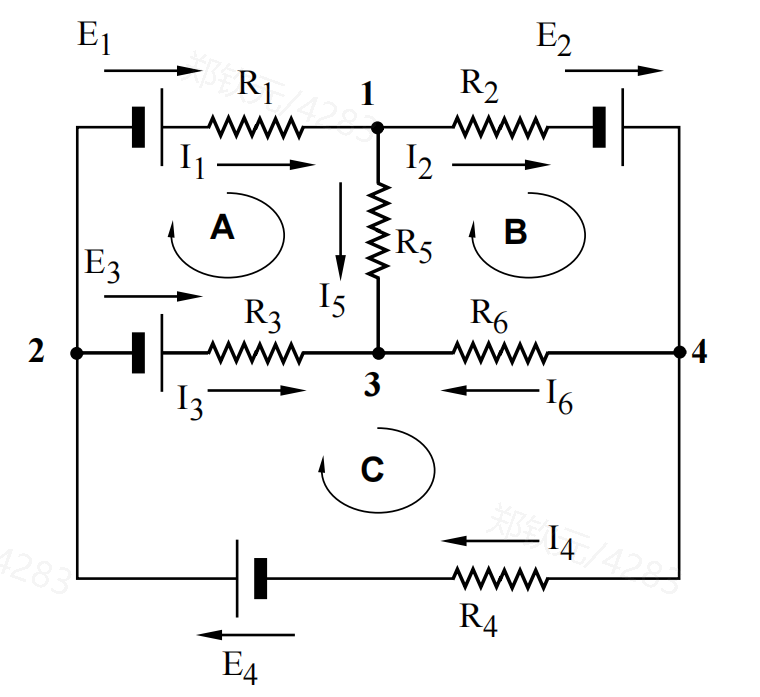
\includegraphics[width=\linewidth]{fig2.6.1} 
    \caption{图2.6.1}
    \label{fig:2.6.1}
\end{figure}

问题是将每个支路中的电流 \(I_k\) 与电阻 \(R_k\) 和电动势 \(E_k\) 联系起来。这可以通过使用欧姆定律结合基尔霍夫定律来产生线性方程组来实现。

\begin{bluebox}{欧姆定律}
欧姆定律指出:对于电流 \(I\) 安培,电阻 \(R\) 欧姆上的电压降(单位:伏特)为 \(V = IR\)。

对于大小为 \(E\) 的EMF源和电流 \(I\),源内部总是有一个小的内阻,其上的电压降为 \(V = E - I \times \text{内阻}\)。但内阻通常可忽略,因此源上的电压降可视为 \(V = E\)。当内阻不可忽略时,其效应可以合并到现有外部电阻中,或视为单独的外部电阻。
\end{bluebox}

\begin{bluebox}{基尔霍夫定律}
\textbf{节点规则:} 流向每个节点的电流的代数和为零。即,总流入电流必须等于总流出电流。这仅仅是电荷守恒的陈述。

\textbf{回路规则:} 每个回路中电动势的代数和必须等于同一回路中 \(IR\) 乘积的代数和。即,假设源内阻已考虑,则源上电压降的代数和等于每个回路中电阻上电压降的代数和。这是能量守恒的陈述。
\end{bluebox}

基尔霍夫定律可以在不知道电流和EMF方向的情况下使用。你可以任意指定方向。如果最终解中出现负值,则实际方向与假设方向相反。应用节点规则时,如果电流方向朝向节点,则视为正;否则视为负。显然,节点规则总是产生齐次方程组。例如,将节点规则应用于图2.6.1中的电路,会产生四个齐次方程,六个未知数(即 \(I_k\)):
\[
\begin{aligned}
&\text{节点1: } I_1 - I_2 - I_5 = 0 \\
&\text{节点2: } I_2 - I_3 - I_4 = 0 \\
&\text{节点3: } I_5 + I_6 - I_1 = 0 \\
&\text{节点4: } I_3 + I_4 - I_6 = 0
\end{aligned}
\]

应用回路规则时,必须选择某个方向(顺时针或逆时针)作为正方向,该方向上的所有EMF和电流视为正,相反方向视为负。一个电流在节点规则中可能被视为正,但在回路规则中使用时可能被视为负。如果正方向被视为顺时针,则将回路规则应用于图2.6.1中的三个指示回路A、B和C,会产生三个非齐次方程,六个未知数(\(I_k\) 视为未知数,而 \(R_k\) 和 \(E_k\) 假设已知):
\[
\begin{aligned}
&\text{回路A: } E_1 - E_2 = I_1 R_1 - I_2 R_2 \\
&\text{回路B: } E_2 = I_2 R_2 + I_3 R_3 + I_4 R_4 \\
&\text{回路C: } E_3 = I_4 R_4 - I_5 R_5 - I_6 R_6
\end{aligned}
\]

还有另外四个回路也会产生回路方程,总共有11个方程(4个节点方程和7个回路方程)和6个未知数。虽然这看起来是一个一般的 \(11 \times 6\) 方程组,但事实并非如此。如果电路处于平衡状态,则物理情况要求对于每组EMF \(E_k\),对应的电流 \(I_k\) 必须唯一确定。换句话说,物理保证由基尔霍夫定律产生的 \(11 \times 6\) 系统必须是一致的且具有唯一解。

假设 \([A \mid b]\) 表示由基尔霍夫定律生成的 \(11 \times 6\) 系统的增广矩阵。从 §2.5 的结果中,我们知道系统有唯一解当且仅当:
\[
\text{rank}(A) = \text{rank}([A \mid b]) = n = 6
\]
此外,§2.3 中证明了系统是一致的当且仅当:
\[
\text{rank}(A) = \text{rank}([A \mid b])
\]
结合这两个事实,我们可以得出结论:
\[
\text{rank}([A \mid b]) = \text{rank}(A) = 6
\]
因此,当 \([A \mid b]\) 被简化为 \(E_{[A \mid b]}\) 时,将恰好有6个非零行和5个零行。因此,原始11个方程中有5个是冗余的,因为它们可以通过特定6个“独立”方程的组合“归零”。最好提前知道11个方程中哪些是冗余的,哪些可以作为“独立”集。

注意,在使用节点规则时,节点4的方程仅仅是节点1、2和3方程的负和,且前三个方程是独立的,即三个方程中没有一个可以写为其他两个的组合。这种情况是典型的。对于具有 \(n\) 个节点的一般电路,可以证明前 \(n-1\) 个节点的方程是独立的,最后一个节点的方程是冗余的。

回路规则也会产生冗余方程。只有简单回路(不包含更小回路的回路)会产生独立方程。例如,考虑图2.6.1中由三个外部支路组成的大回路。将回路规则应用于这个大回路不会产生新信息,因为大回路可以通过“加”其内部的三个简单回路A、B和C来构造。与大外部回路相关的方程为:
\[
E_1 - E_2 + E_3 = I_1 R_1 - I_2 R_2 + I_3 R_3 + I_4 R_4 - I_5 R_5 - I_6 R_6
\]
这正好是对应三个组成回路A、B和C的方程之和。这种现象在一般情况下成立,因此使用回路规则时只需考虑简单回路。

讨论的要点是结论:更一般的 \(11 \times 6\) 矩形系统可以通过丢弃最后一个节点方程并仅使用简单回路方程,替换为等效的 \(6 \times 6\) 平方系统,该系统具有唯一解。这是实际工作的典型特征。问题的物理性质连同自然约束通常可用于将一般矩形系统替换为平方且具有唯一解的系统。

我们研究的目标之一是更清楚地理解此应用中出现的“独立性”概念。到目前为止,独立性是一个直观概念,但此示例有助于阐明独立性是一个基本重要概念,值得更牢固地确定。这将在§4.3中完成,并且从电路获得独立方程的一般理论在示例4.4.6和4.4.7中开发。

\textcolor{red}{练习2.6}
\color{red}\rule{\textwidth}{0.4pt}\color{black}

\begin{enumerate}[leftmargin=*, label=\bfseries 2.6.\arabic*]
    \item 假设在图2.6.1所示的电路中,\(R_i = i\) 欧姆,\(E_i = i\) 伏特。
    \begin{enumerate}[label=(\alph*)]
        \item 确定六个指示电流。
        \item 选择节点1作为参考点,并将其电位固定为0伏特。相对于此参考,计算其他三个节点的电位。通过验证每个回路的回路规则来检查你的答案。
    \end{enumerate}

    \item 确定以下电路中的三个指示电流。
    \begin{figure}[h]
        \centering
        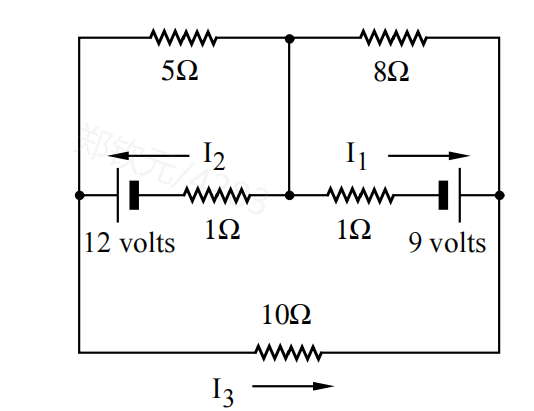
\includegraphics[width=\linewidth]{fig2.6.2} 
        \caption{图2.6.2}
        \label{fig:2.6.2}
    \end{figure}

    \item 确定以下电路中的两个未知EMF。
    \begin{figure}[h]
        \centering
        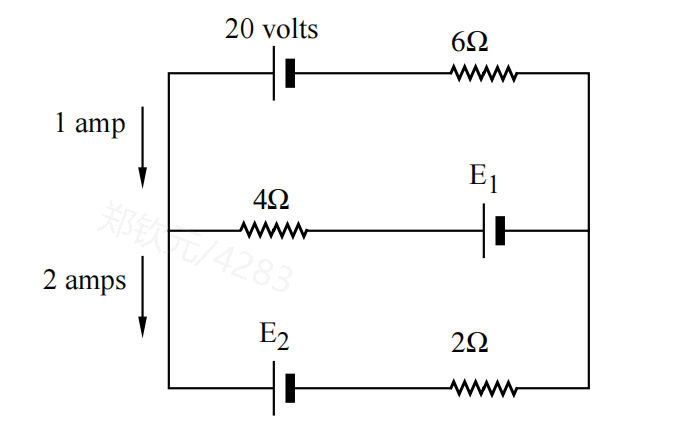
\includegraphics[width=\linewidth]{fig2.6.3} 
        \caption{图2.6.3}
        \label{fig:2.6.3}
    \end{figure}

    \item 考虑以下所示电路并回答以下问题。
    \begin{figure}[h]
        \centering
        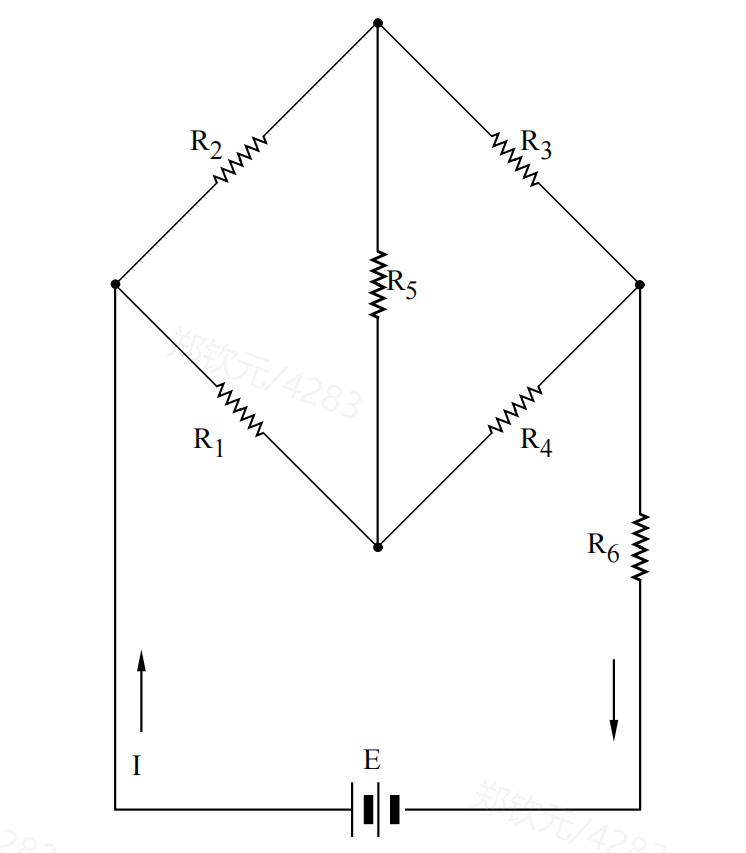
\includegraphics[width=\linewidth]{fig2.6.4} 
        \caption{图2.6.4}
        \label{fig:2.6.4}
    \end{figure}
    \begin{enumerate}[label=(\alph*)]
        \item 电路包含多少个节点?
        \item 电路包含多少个支路?
        \item 确定回路的总数,然后确定简单回路的数量。
        \item 证明简单回路方程形成“独立”方程组,即没有冗余方程。
        \item 验证任何三个节点方程构成“独立”方程组。
        \item 验证与包含 \(R_1, R_2, R_3, R_4\) 的回路相关的回路方程可以表示为包含在较大回路中的两个简单回路的两个方程之和。
        \item 如果 \(R_1 = R_2 = R_3 = R_4 = 1\) 欧姆,\(R_5 = R_6 = 5\) 欧姆,且 \(E = 5\) 伏特,确定指示电流 \(I\)。
    \end{enumerate}
\end{enumerate}


\end{document}